\documentclass[12pt,a4paper]{article}

% ===== Codificación y español =====
\usepackage[utf8]{inputenc}
\usepackage[T1]{fontenc}
\usepackage[spanish, es-tabla]{babel}

% ===== Márgenes y gráficos =====
\usepackage{geometry}
\geometry{margin=2.5cm}
\usepackage{graphicx}
\usepackage{float}        % [H] para fijar figuras/tablas
\usepackage{subcaption}   % subfiguras
\usepackage{booktabs}     % tablas más bonitas

% ===== Hipervínculos y referencias =====
\usepackage{hyperref}
\hypersetup{
  colorlinks=true,
  linkcolor=black,
  citecolor=black,
  urlcolor=blue
}

\usepackage{siunitx}
\sisetup{
  output-decimal-marker = {.}, % decimal con punto
  group-separator = {,},       % miles con coma
  group-minimum-digits = 4,
  group-digits = integer,
  table-number-alignment = center,
  round-mode = places,
  detect-all = true            % ignora configuraciones de babel
}


% cleveref mejora \ref: escribe "Figura 1", "Tabla 2", etc.
\usepackage[capitalise,noabbrev]{cleveref}

% Ajuste de nombres en cleveref
\crefname{figure}{figura}{figuras}
\Crefname{figure}{Figura}{Figuras}
\crefname{subfigure}{subfigura}{subfiguras}
\Crefname{subfigure}{Subfigura}{Subfiguras}
\crefname{table}{tabla}{tablas}
\Crefname{table}{Tabla}{Tablas}
\crefname{equation}{ecuación}{ecuaciones}
\Crefname{equation}{Ecuación}{Ecuaciones}
\crefname{section}{sección}{secciones}
\Crefname{section}{Sección}{Secciones}

% Listas más controlables
\usepackage{enumitem}

\graphicspath{{figures/}}
\usepackage{adjustbox}


% ===== Título y autoría =====
\title{\textbf{Informe del análisis de datos para el dataset ``Adult''}}
\author{Haessler Joan Ortiz Moncada \\[0.5cm]
        Universidad Distrital Francisco José de Caldas \\
        Facultad de Ingeniería \\
        Curso: Big Data}
\date{\today}

\begin{document}

\maketitle

\section{Introducción}
El \textit{Adult Income Dataset}, también conocido como \textit{Census Income Dataset}, 
proviene del Censo de 1994 de Estados Unidos. El objetivo típico de estudio es predecir 
si una persona gana más de \num{50000} dólares anuales a partir de características demográficas 
y socioeconómicas. Es un conjunto de datos ampliamente utilizado en problemas de clasificación supervisada.

\section{Metodología}
Se emplearon Google Colab y Python con las librerías \texttt{pandas}, \texttt{scikit-learn}, 
\texttt{matplotlib} y \texttt{seaborn}. Los resultados, figuras y tablas se documentan en \LaTeX.

\section{Descripción del dataset}
El conjunto de datos contiene \num{48842} registros, distribuidos en dos archivos: 
\texttt{adult.data} (con \num{32561} instancias) y \texttt{adult.test} (con \num{16281} instancias). 
Incluye 14 características y una variable objetivo denominada \texttt{income}. 
La \Cref{tab:adult_attributes} presenta los campos y su tipo.

\subsection{Atributos del dataset}

\begin{table}[H]
  \centering
  \begin{tabular}{@{}ll@{}}
    \toprule
    \textbf{Atributo} & \textbf{Tipo} \\ \midrule
    \texttt{age}             & Numérico (int64) \\
    \texttt{workclass}       & Categórico \\
    \texttt{fnlwgt}          & Numérico (int64) \\
    \texttt{education}       & Categórico \\
    \texttt{education-num}   & Numérico (int64) \\
    \texttt{marital-status}  & Categórico \\
    \texttt{occupation}      & Categórico \\
    \texttt{relationship}    & Categórico \\
    \texttt{race}            & Categórico \\
    \texttt{sex}             & Categórico \\
    \texttt{capital-gain}    & Numérico (int64) \\
    \texttt{capital-loss}    & Numérico (int64) \\
    \texttt{hours-per-week}  & Numérico (int64) \\
    \texttt{native-country}  & Categórico \\
    \texttt{income}          & Categórico (objetivo) \\ \bottomrule
  \end{tabular}
  \caption{Atributos y tipo de dato}
  \label{tab:adult_attributes}
\end{table}

Para este informe se unificaron ambos archivos en un único \emph{DataFrame}. La división 
original probablemente busca facilitar la replicación de resultados entre entrenamiento y 
prueba. El repositorio incluye, además, el dominio de cada característica y documentación 
de tipos.

\section{Resultados y análisis}
A continuación se sigue la estructura del \textit{Assignment \#2} del curso de Big Data.

\begin{enumerate}
   \item \textbf{Q1: Exploración y análisis de datos}
    \begin{itemize}
      \item \textbf{Estadísticas descriptivas} para variables numéricas:
      \begin{table}[H]
        \centering
        \small
        \begin{tabular}{@{}l S[table-format=2.2] S[table-format=6.2] S[table-format=2.2] S[table-format=5.2] S[table-format=4.2] S[table-format=2.2]@{}}
          \toprule
          \textbf{Estadístico} & \textbf{age} & \textbf{fnlwgt} & \textbf{education-num} & \textbf{capital-gain} & \textbf{capital-loss} & \textbf{hours-per-week} \\
          \midrule
          count & 48842.00 & 48842.00 & 48842.00 & 48842.00 & 48842.00 & 48842.00 \\
          mean  & 38.64    & 189664.13 & 10.08    & 1079.07  & 87.50    & 40.42 \\
          std   & 13.71    & 105604.03 & 2.57     & 7452.02  & 403.00   & 12.39 \\
          min   & 17.00    & 12285.00  & 1.00     & 0.00     & 0.00     & 1.00 \\
          25\%  & 28.00    & 117550.50 & 9.00     & 0.00     & 0.00     & 40.00 \\
          50\%  & 37.00    & 178144.50 & 10.00    & 0.00     & 0.00     & 40.00 \\
          75\%  & 48.00    & 237642.00 & 12.00    & 0.00     & 0.00     & 45.00 \\
          max   & 90.00    & 1490400.00& 16.00    & 99999.00 & 4356.00  & 99.00 \\
          \bottomrule
        \end{tabular}
        \caption{Estadísticas descriptivas de variables numéricas}
        \label{tab:adult_stats}
      \end{table}
    \end{itemize}

    El conjunto presenta seis variables numéricas con comportamientos diversos. En cuanto a tendencia central y 
    dispersión, \texttt{age} tiene una media de 38.64 y mediana de 37, lo que indica un leve sesgo a la derecha. 
    La variable \texttt{hours-per-week} muestra una mediana de 40 y el tercer cuartil en 45, consistente con jornadas 
    laborales estándar y cierta variabilidad. \texttt{education-num} es discreta, centrada en 10 años (Q3 en 12). 
    Por otro lado, \texttt{fnlwgt} exhibe una varianza muy alta y una cola derecha pronunciada. Tanto \texttt{capital-gain} 
    como \texttt{capital-loss} presentan valores extremadamente bajos (Q1=Q2=Q3=0), lo que implica que al menos el 75\,\% de 
    los registros no reportan ganancias ni pérdidas de capital.

    Antes de graficar, se detectó que la variable \texttt{income} tenía cuatro etiquetas distintas por un 
    error de tipeo: algunas instancias presentaban un punto al final (\texttt{<=50K.}, \texttt{>50K.}). Este problema se 
    corrigió unificando las etiquetas en solo dos categorías válidas: \texttt{<=50K} y \texttt{>50K}. A continuación se 
    muestran histogramas y diagramas de caja (\textit{boxplots}) para explorar la distribución de las variables numéricas y 
    la frecuencia de la variable objetivo \texttt{income}.

    % Histograma y boxplot: age
    \begin{figure}[H]
      \centering
      \begin{subfigure}[b]{0.45\textwidth}
        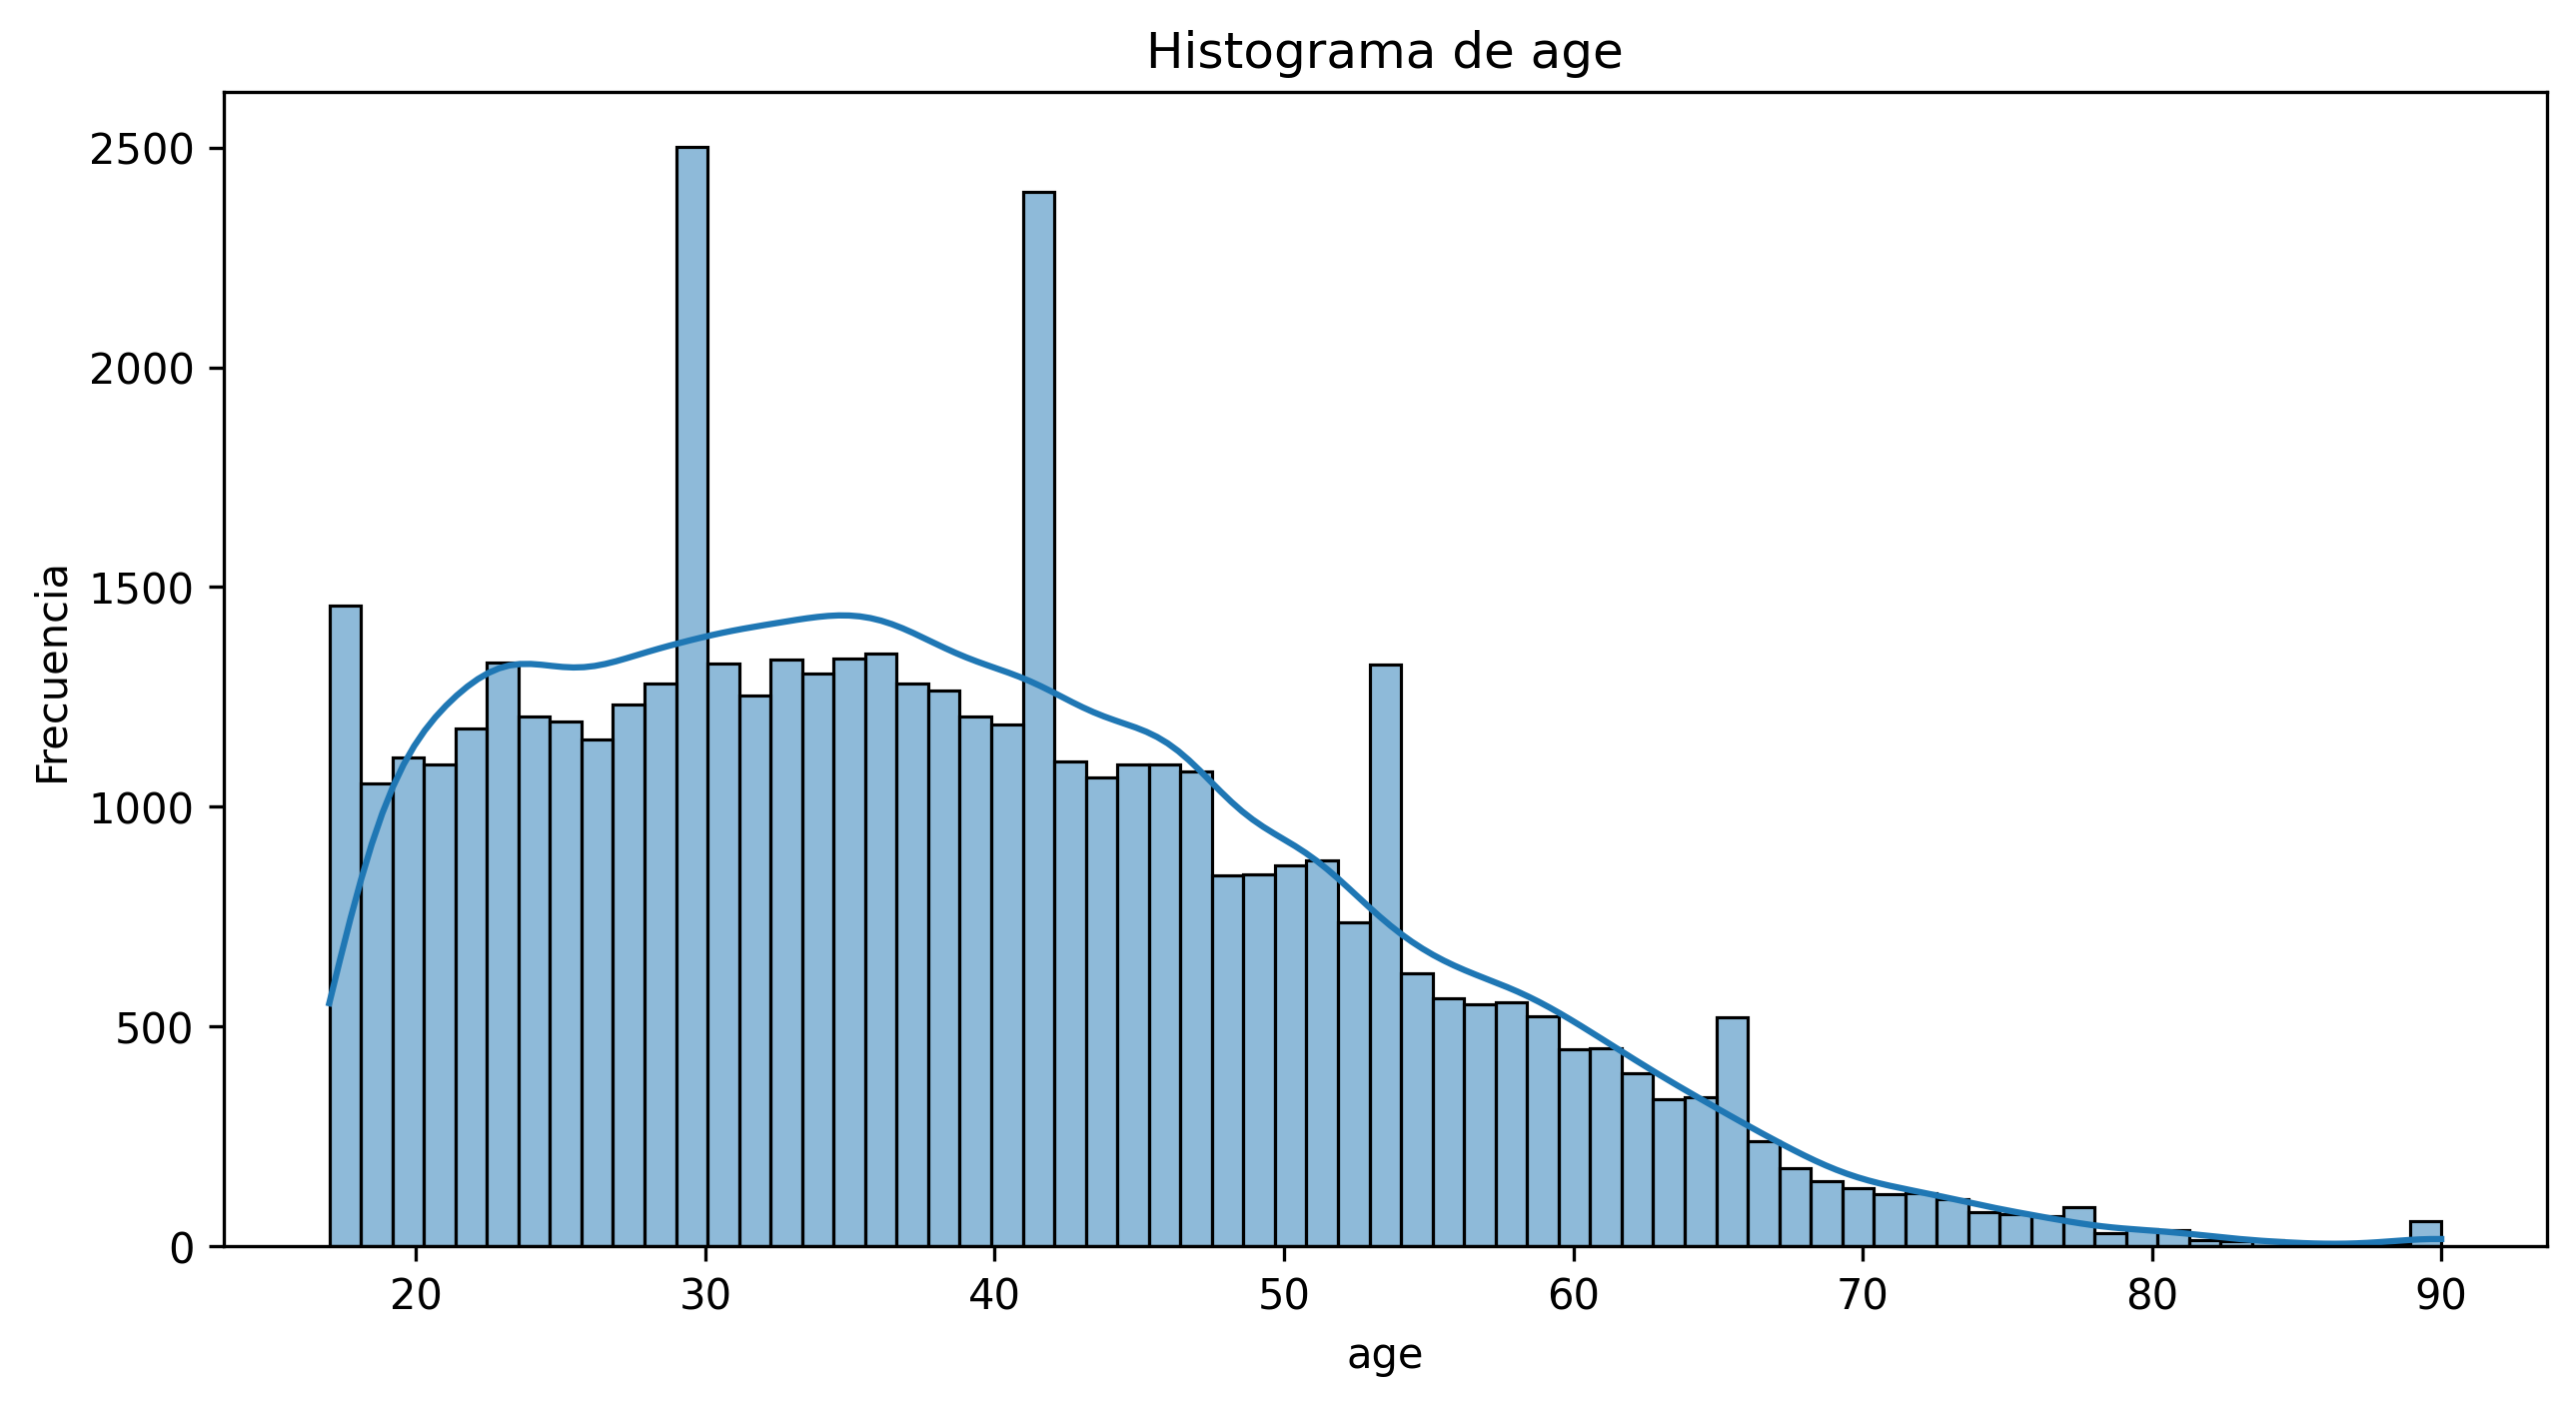
\includegraphics[width=\textwidth]{histogram_age.png}
        \caption{Histograma de \texttt{age}}
        \label{fig:age_hist}
      \end{subfigure}
      \hfill
      \begin{subfigure}[b]{0.45\textwidth}
        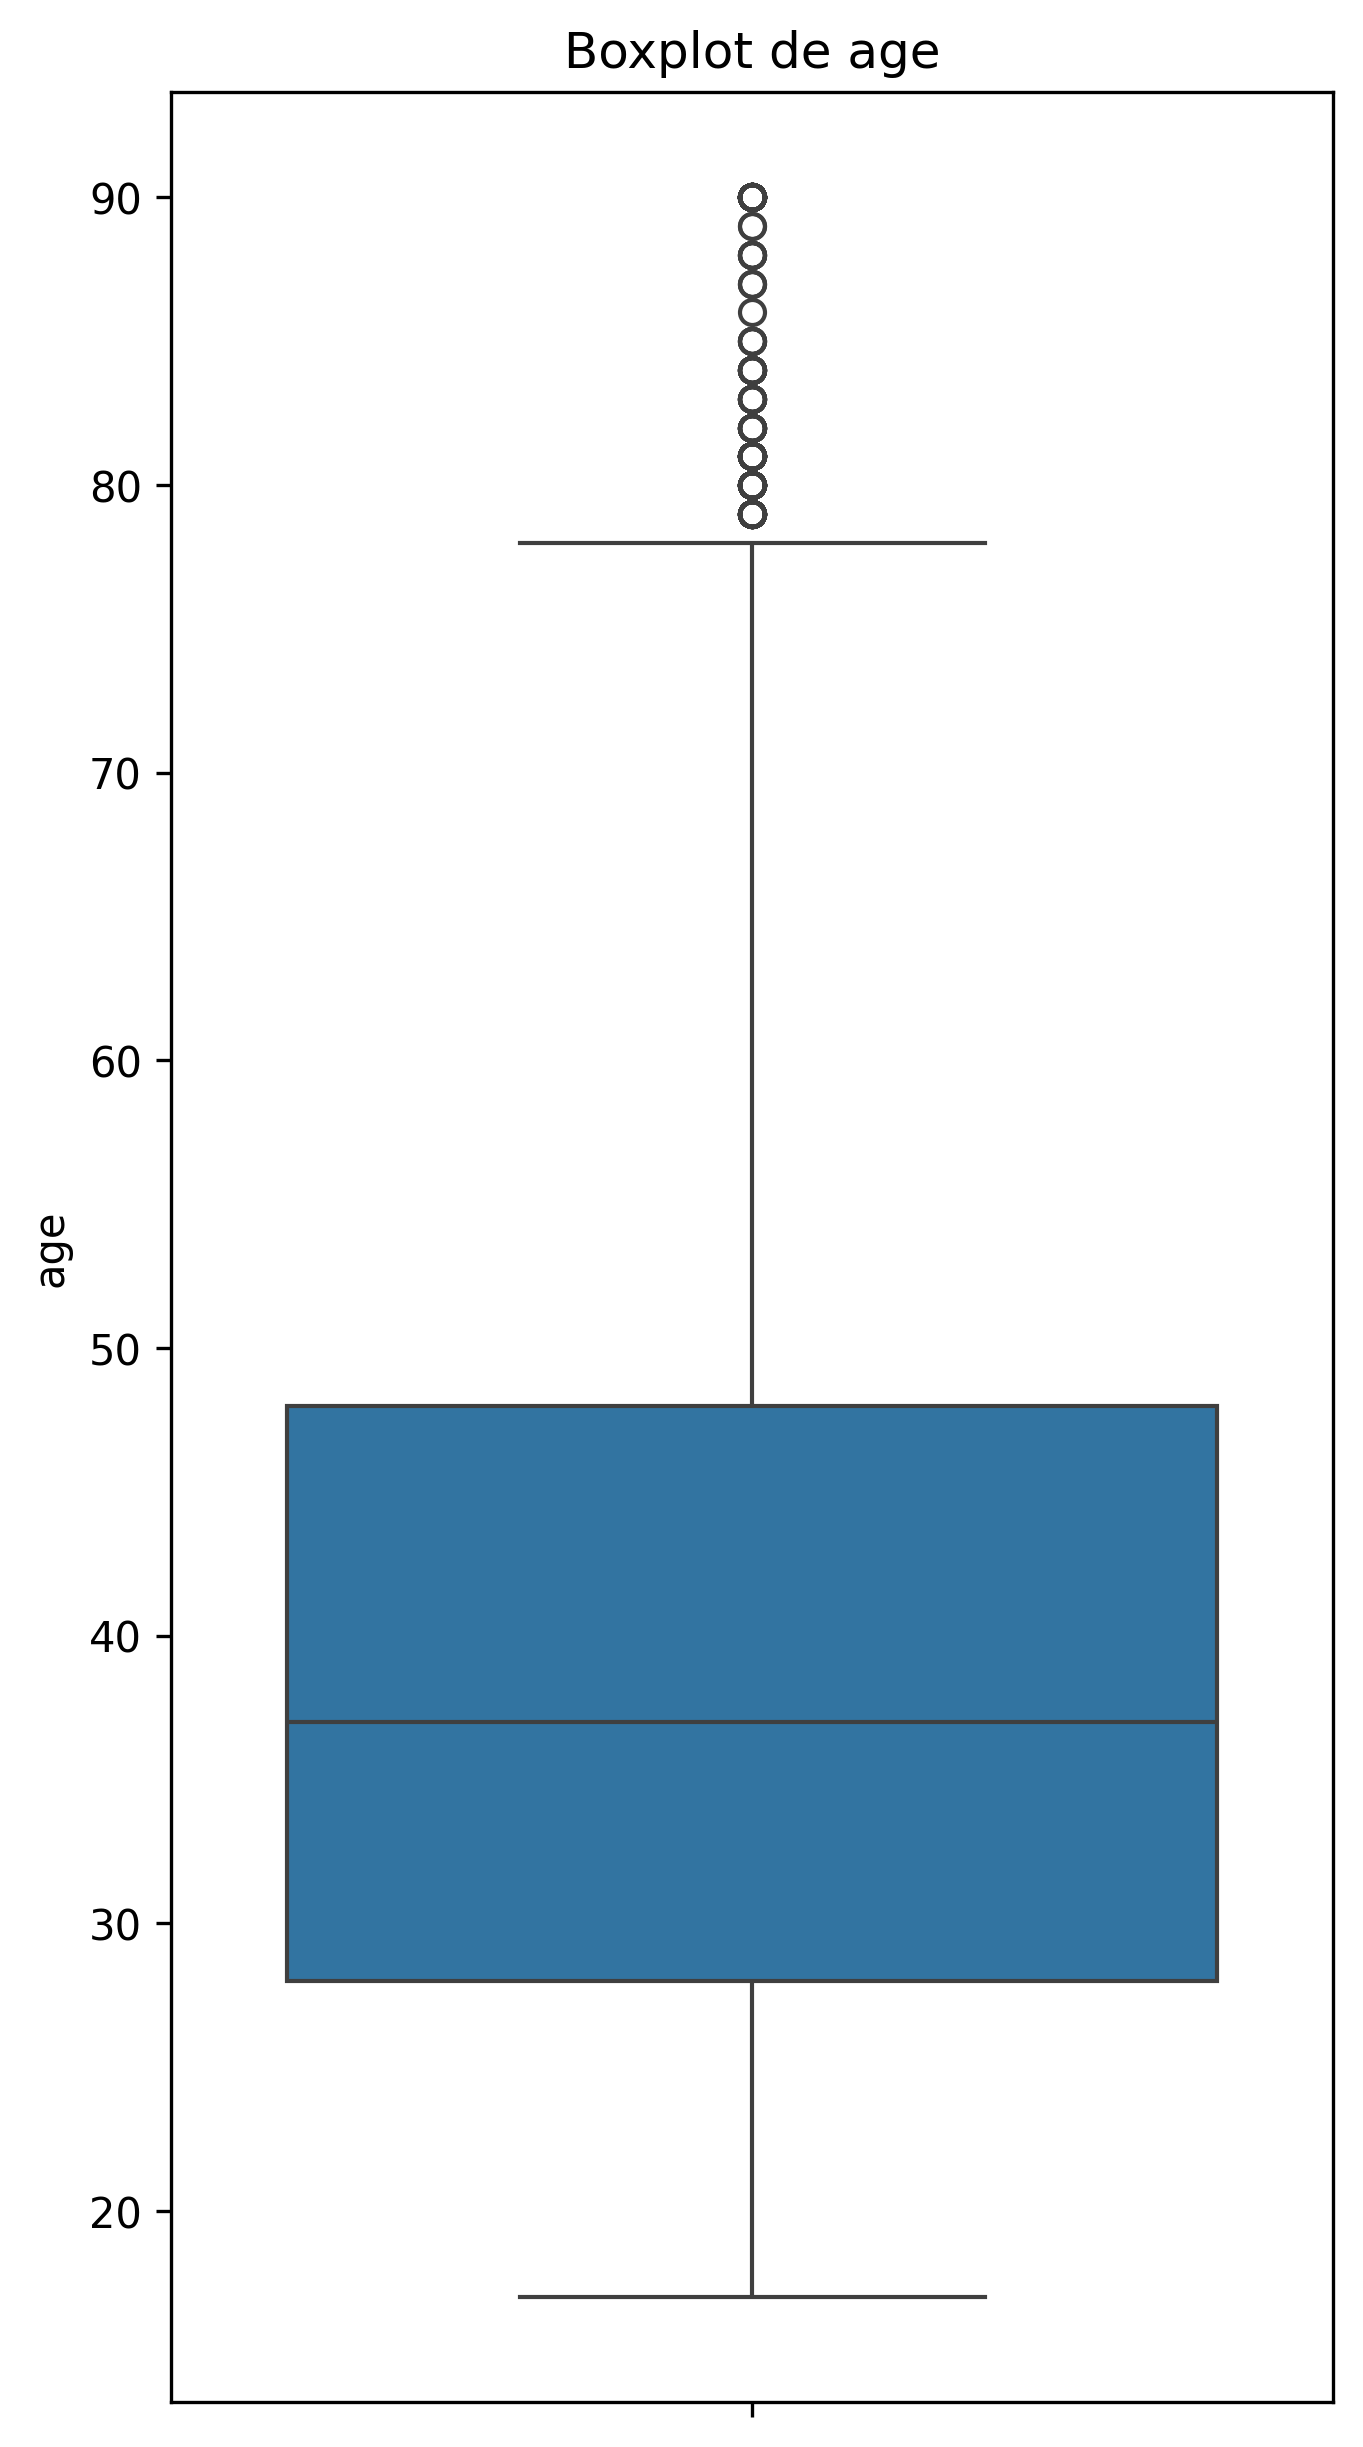
\includegraphics[width=\textwidth]{boxplot_age.png}
        \caption{Boxplot de \texttt{age}}
        \label{fig:age_boxplot}
      \end{subfigure}
      \caption{Distribución de \texttt{age}: histograma y boxplot.}
      \label{fig:age_visual}
    \end{figure}

    La distribución de \emph{age} se concentra entre los 28 y 48 años (rango intercuartílico), con mínimos en 17 
    y máximos en 90. El histograma muestra una mayor densidad entre los 30–50 años y el boxplot revela algunos 
    valores altos atípicos, esperables en poblaciones laborales amplias.

    % Histograma y boxplot: capital-gain
    \begin{figure}[H]
      \centering
      \begin{subfigure}[b]{0.45\textwidth}
        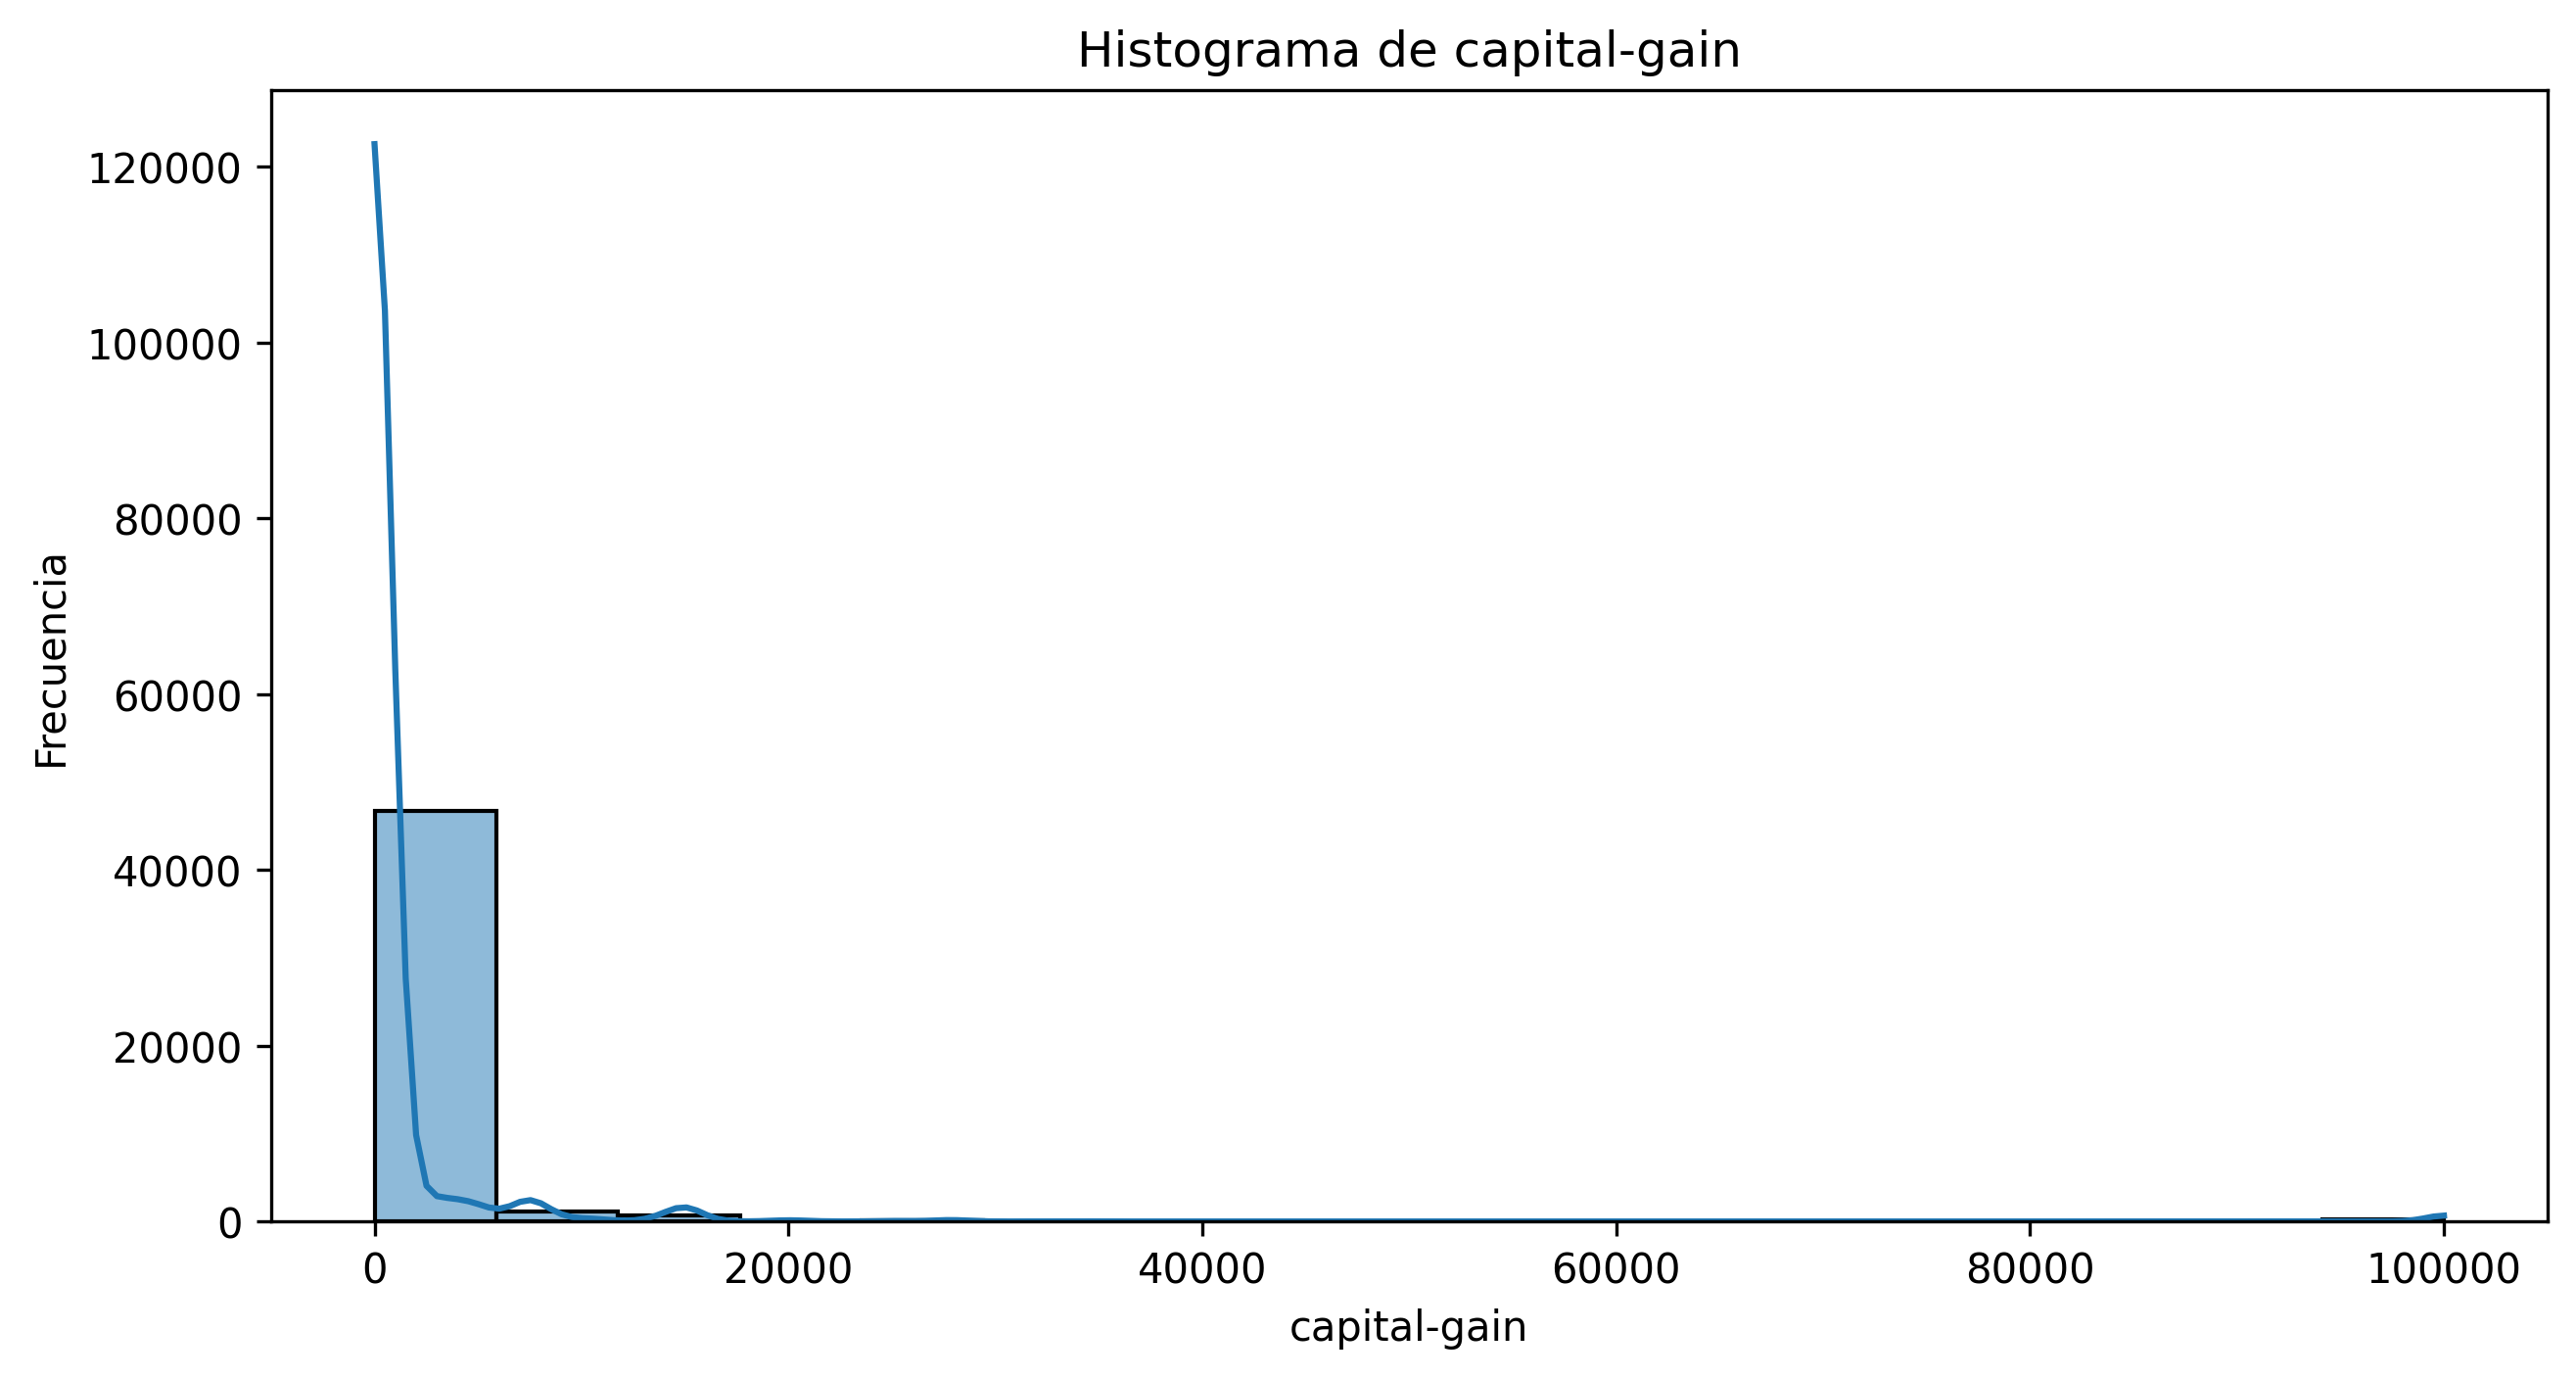
\includegraphics[width=\textwidth]{histogram_capital-gain.png}
        \caption{Histograma de \texttt{capital-gain}}
        \label{fig:capital_gain_hist}
      \end{subfigure}
      \hfill
      \begin{subfigure}[b]{0.45\textwidth}
        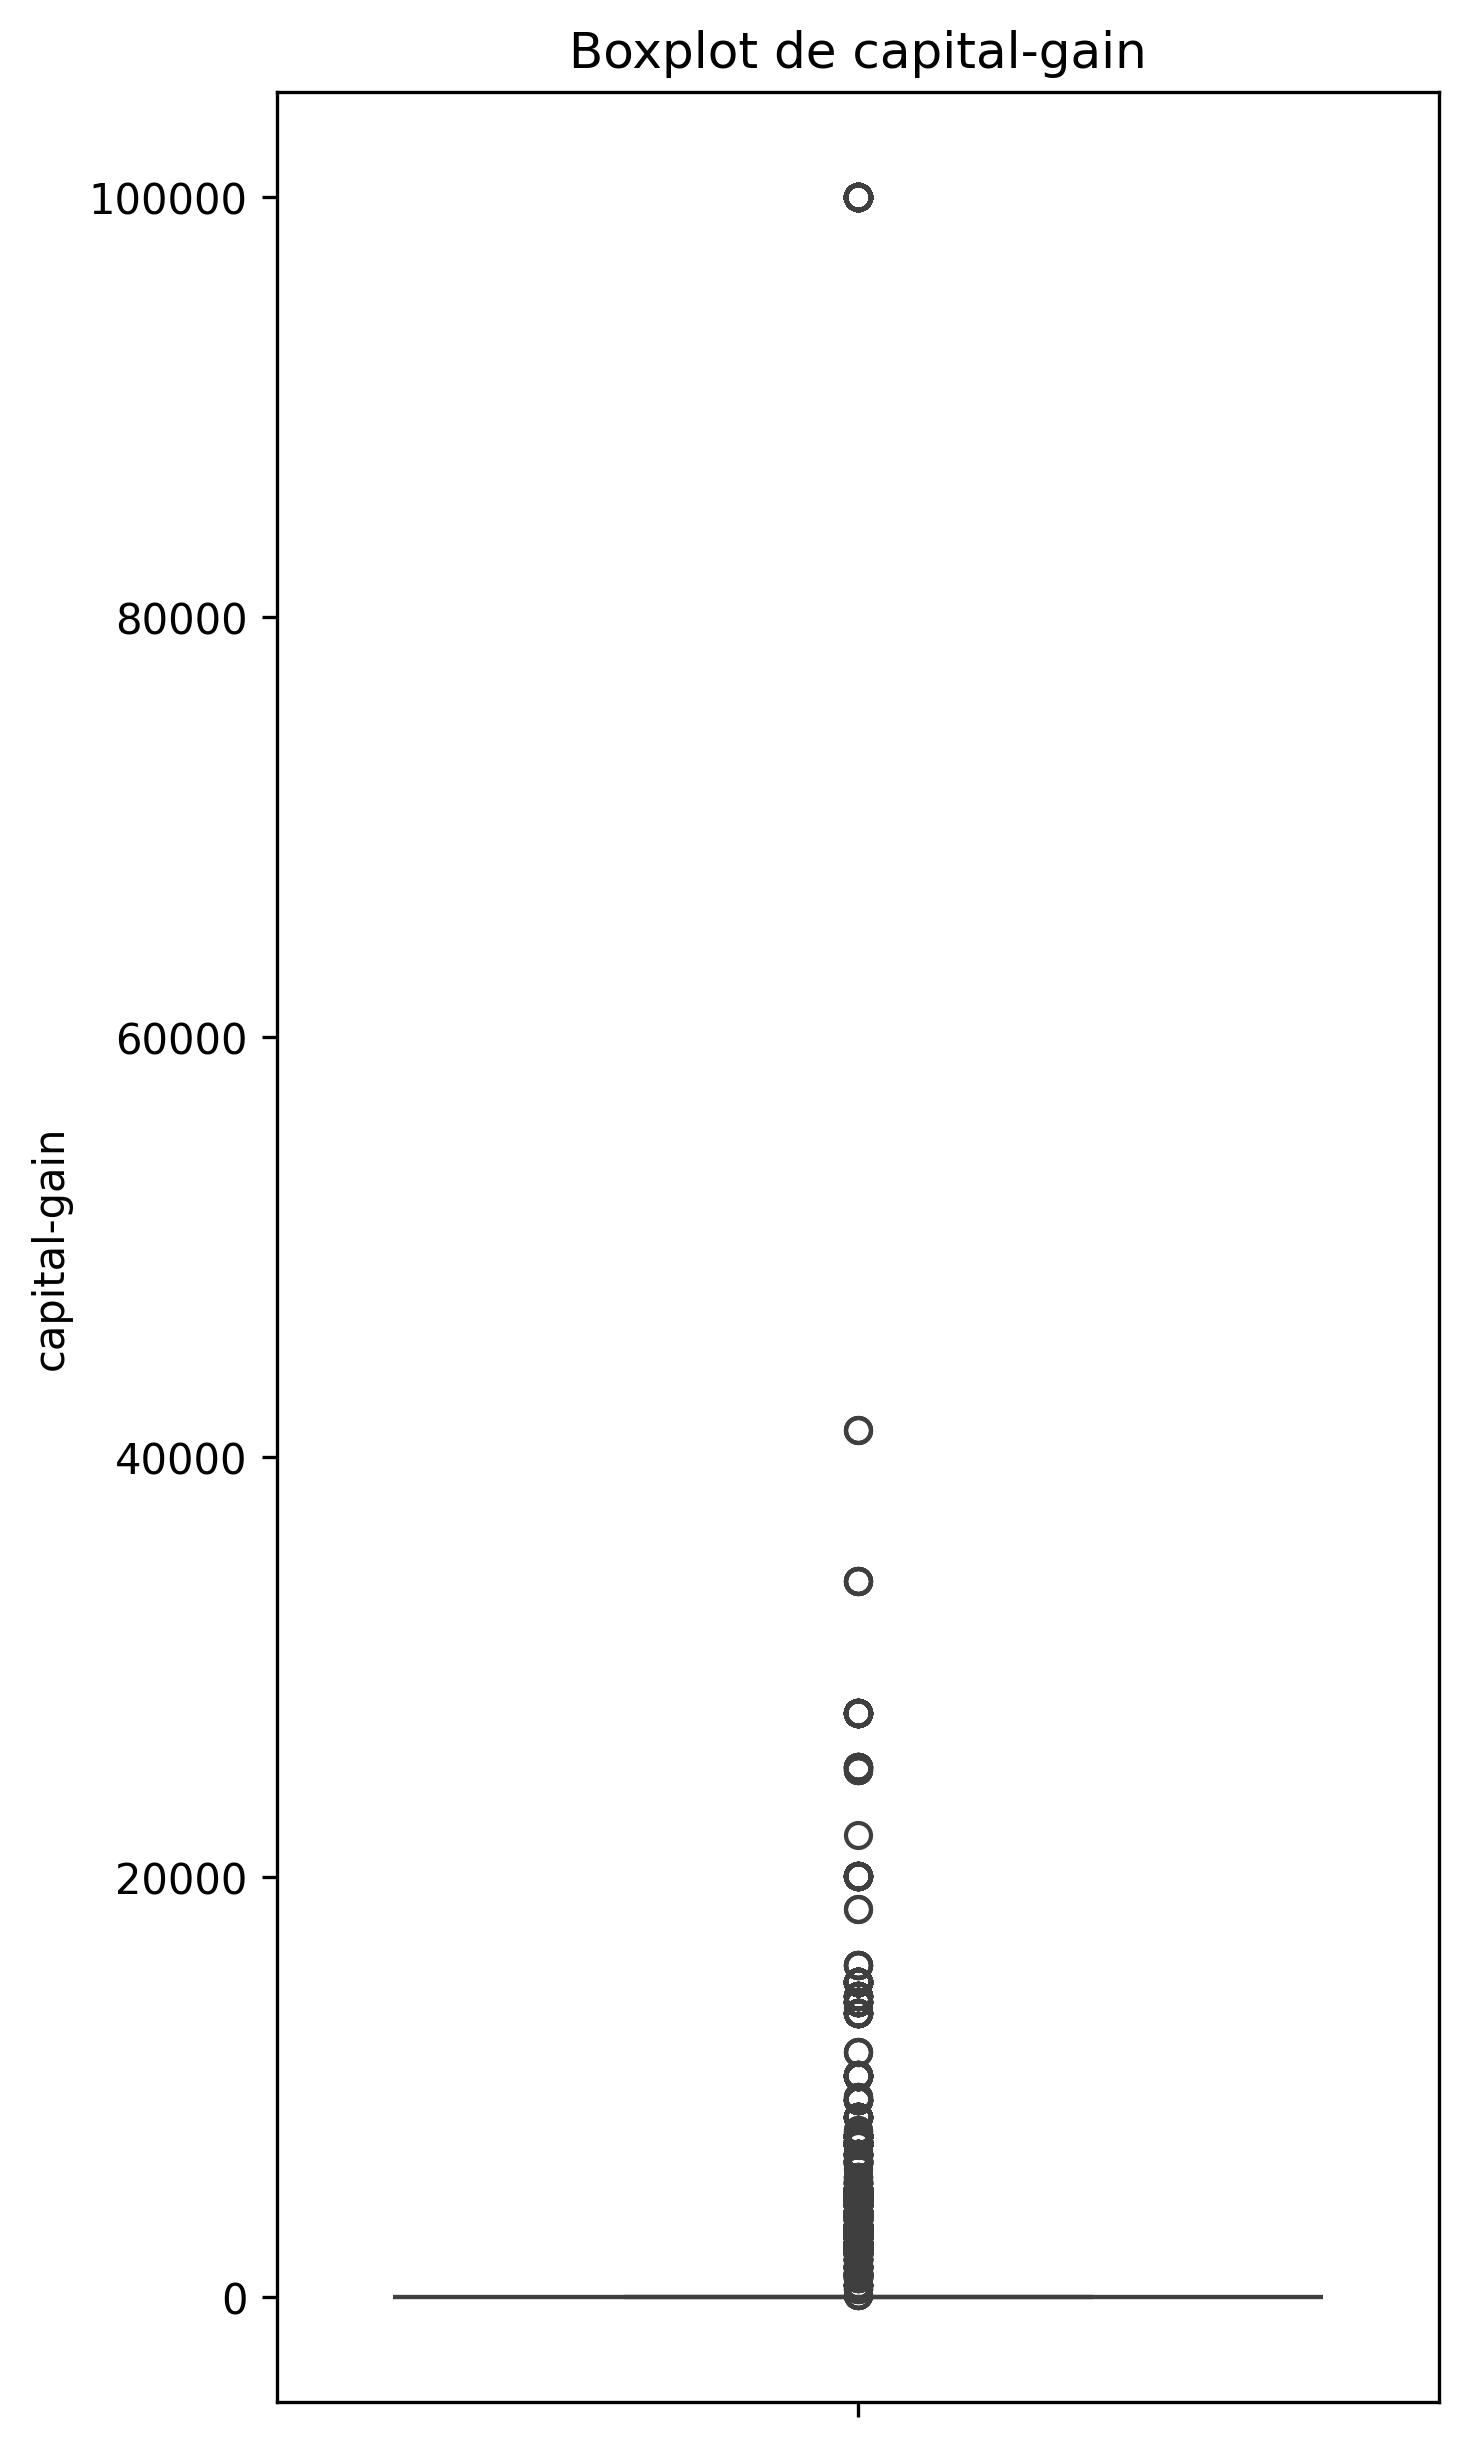
\includegraphics[width=\textwidth]{boxplot_capital-gain.png}
        \caption{Boxplot de \texttt{capital-gain}}
        \label{fig:capital_gain_boxplot}
      \end{subfigure}
      \caption{Distribución de \texttt{capital-gain}: histograma y boxplot.}
      \label{fig:capital_gain_visual}
    \end{figure}

    \emph{capital-gain} está fuertemente sesgada a la derecha: tres cuartiles en cero y una larga cola hasta 
    99,999. El boxplot evidencia numerosos ceros y pocos valores extremadamente altos; el histograma muestra 
    acumulación en cero con muy pocas observaciones en los rangos altos. Esto indica que la mayoría de personas 
    no reportan ganancias de capital, y solo un pequeño grupo tiene valores elevados. Podría convenir aplicar una 
    transformación logarítmica para reducir la asimetría y estabilizar la varianza.

    % Histograma y boxplot: capital-loss
    \begin{figure}[H]
      \centering
      \begin{subfigure}[b]{0.45\textwidth}
        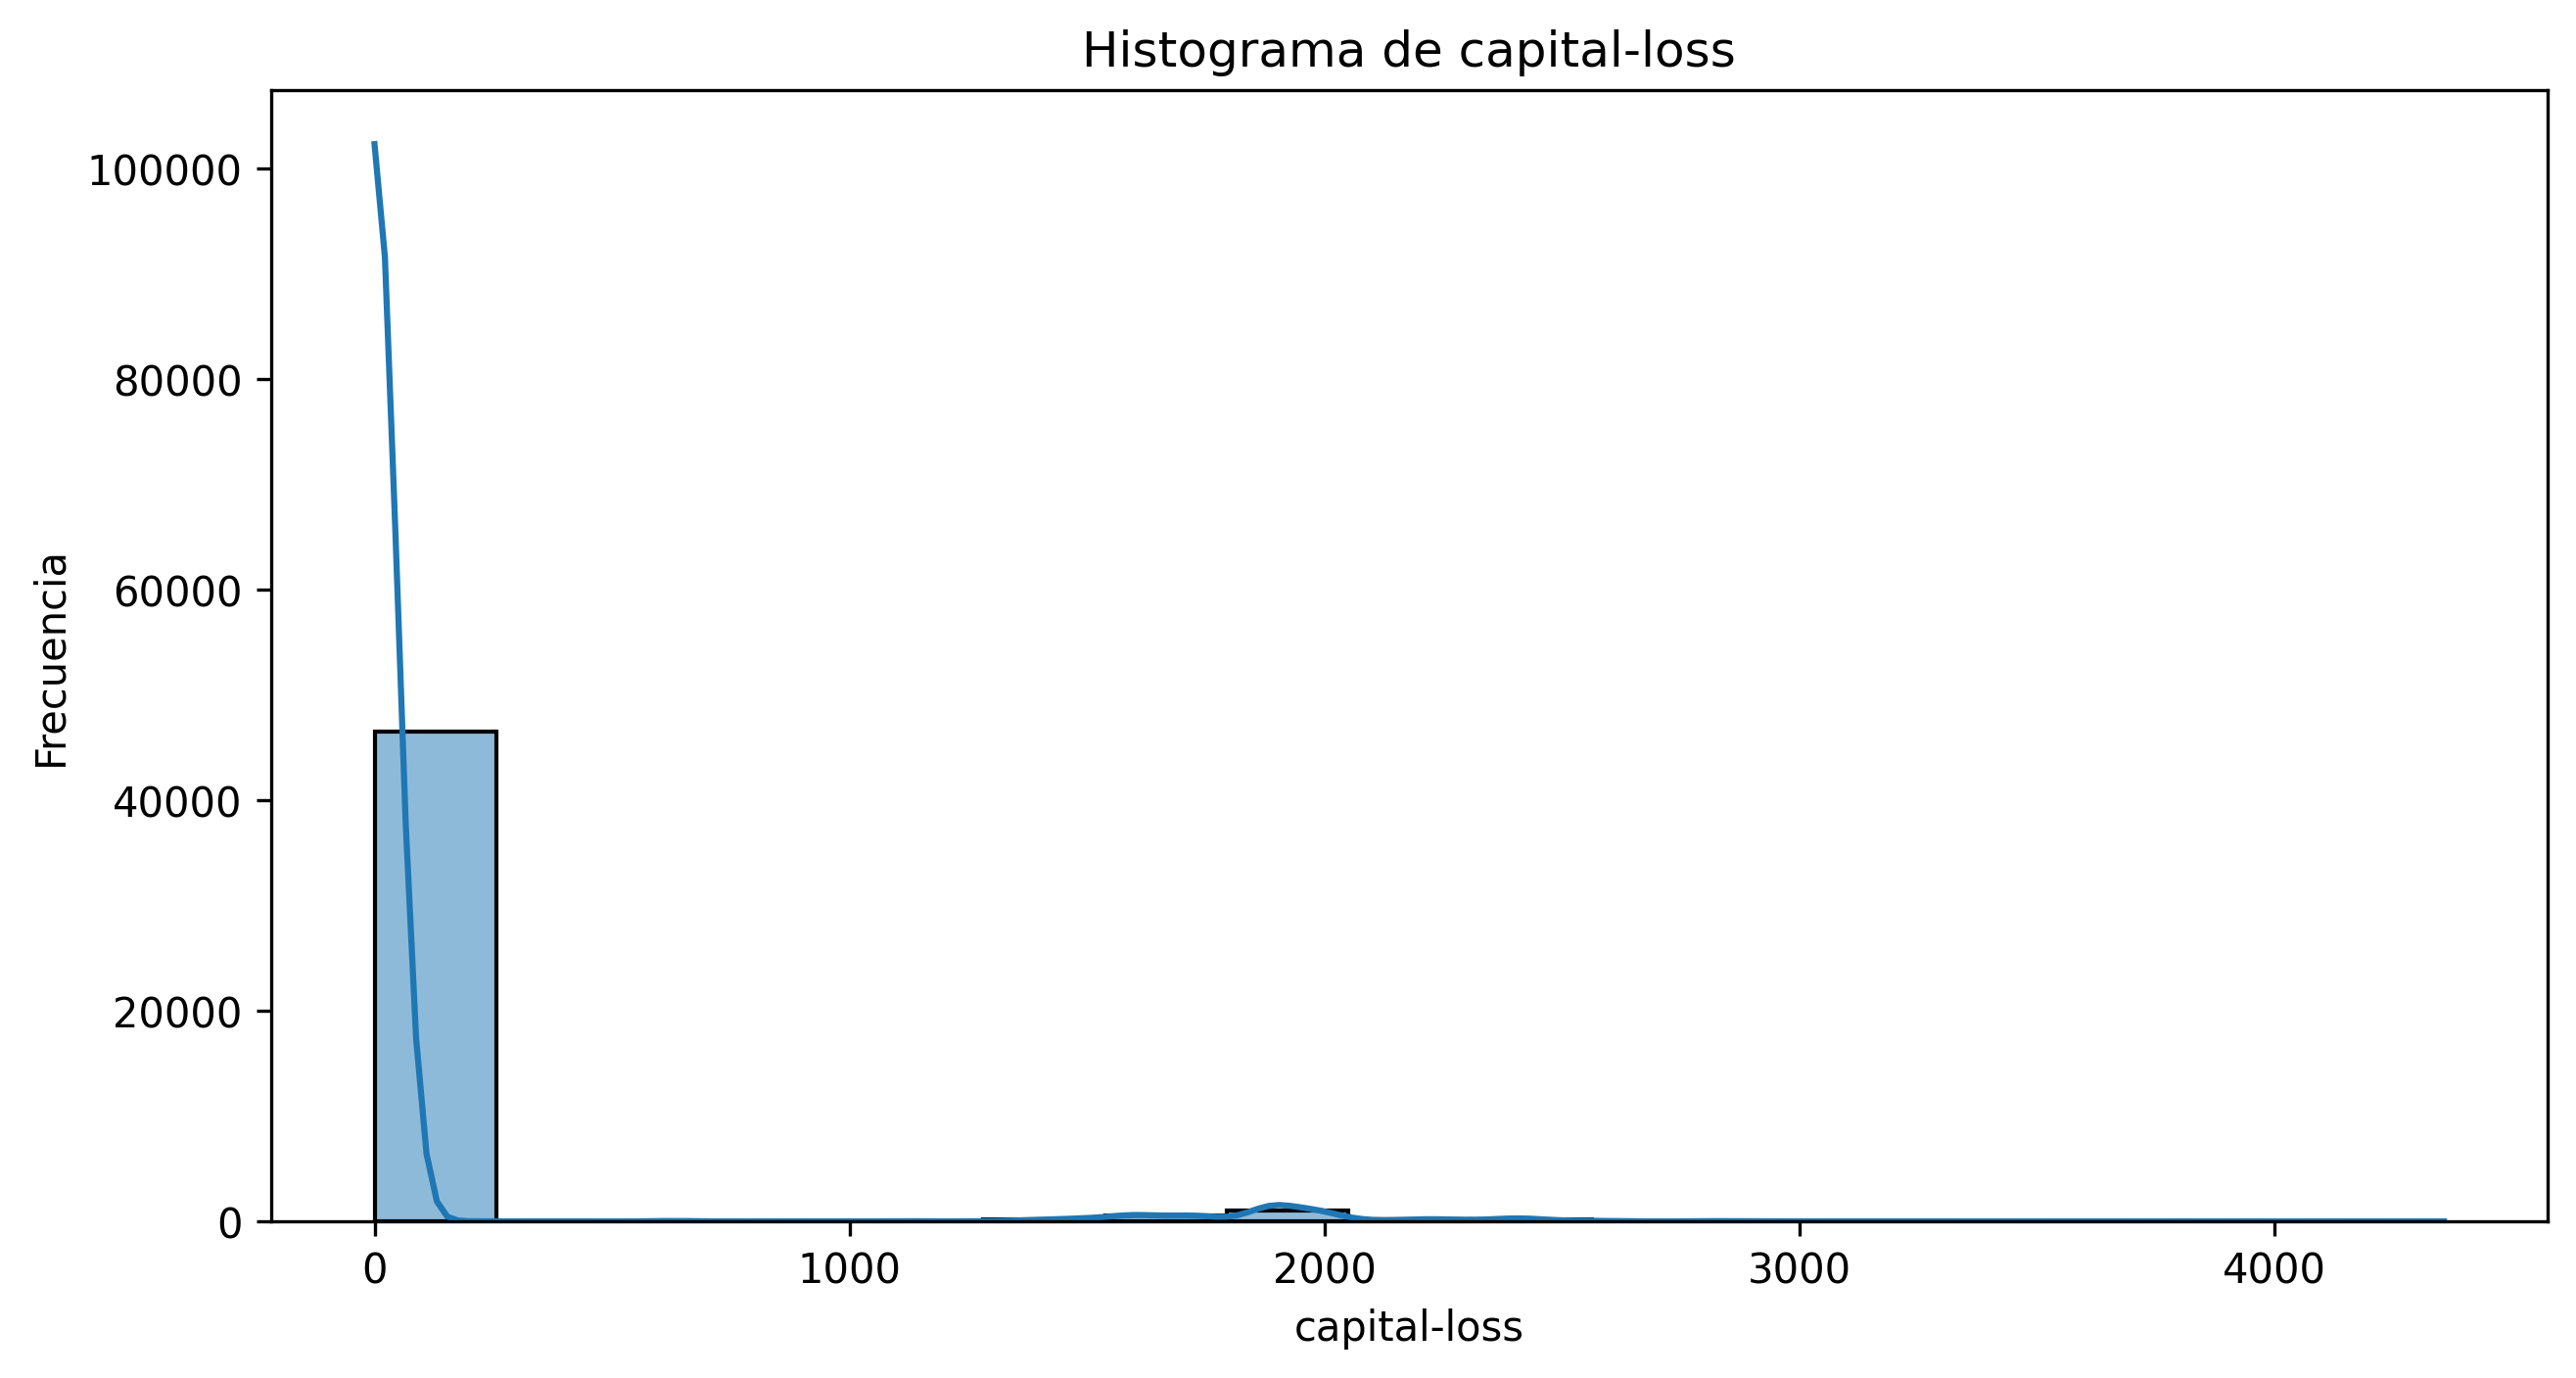
\includegraphics[width=\textwidth]{histogram_capital-loss.png}
        \caption{Histograma de \texttt{capital-loss}}
        \label{fig:capital_loss_hist}
      \end{subfigure}
      \hfill
      \begin{subfigure}[b]{0.45\textwidth}
        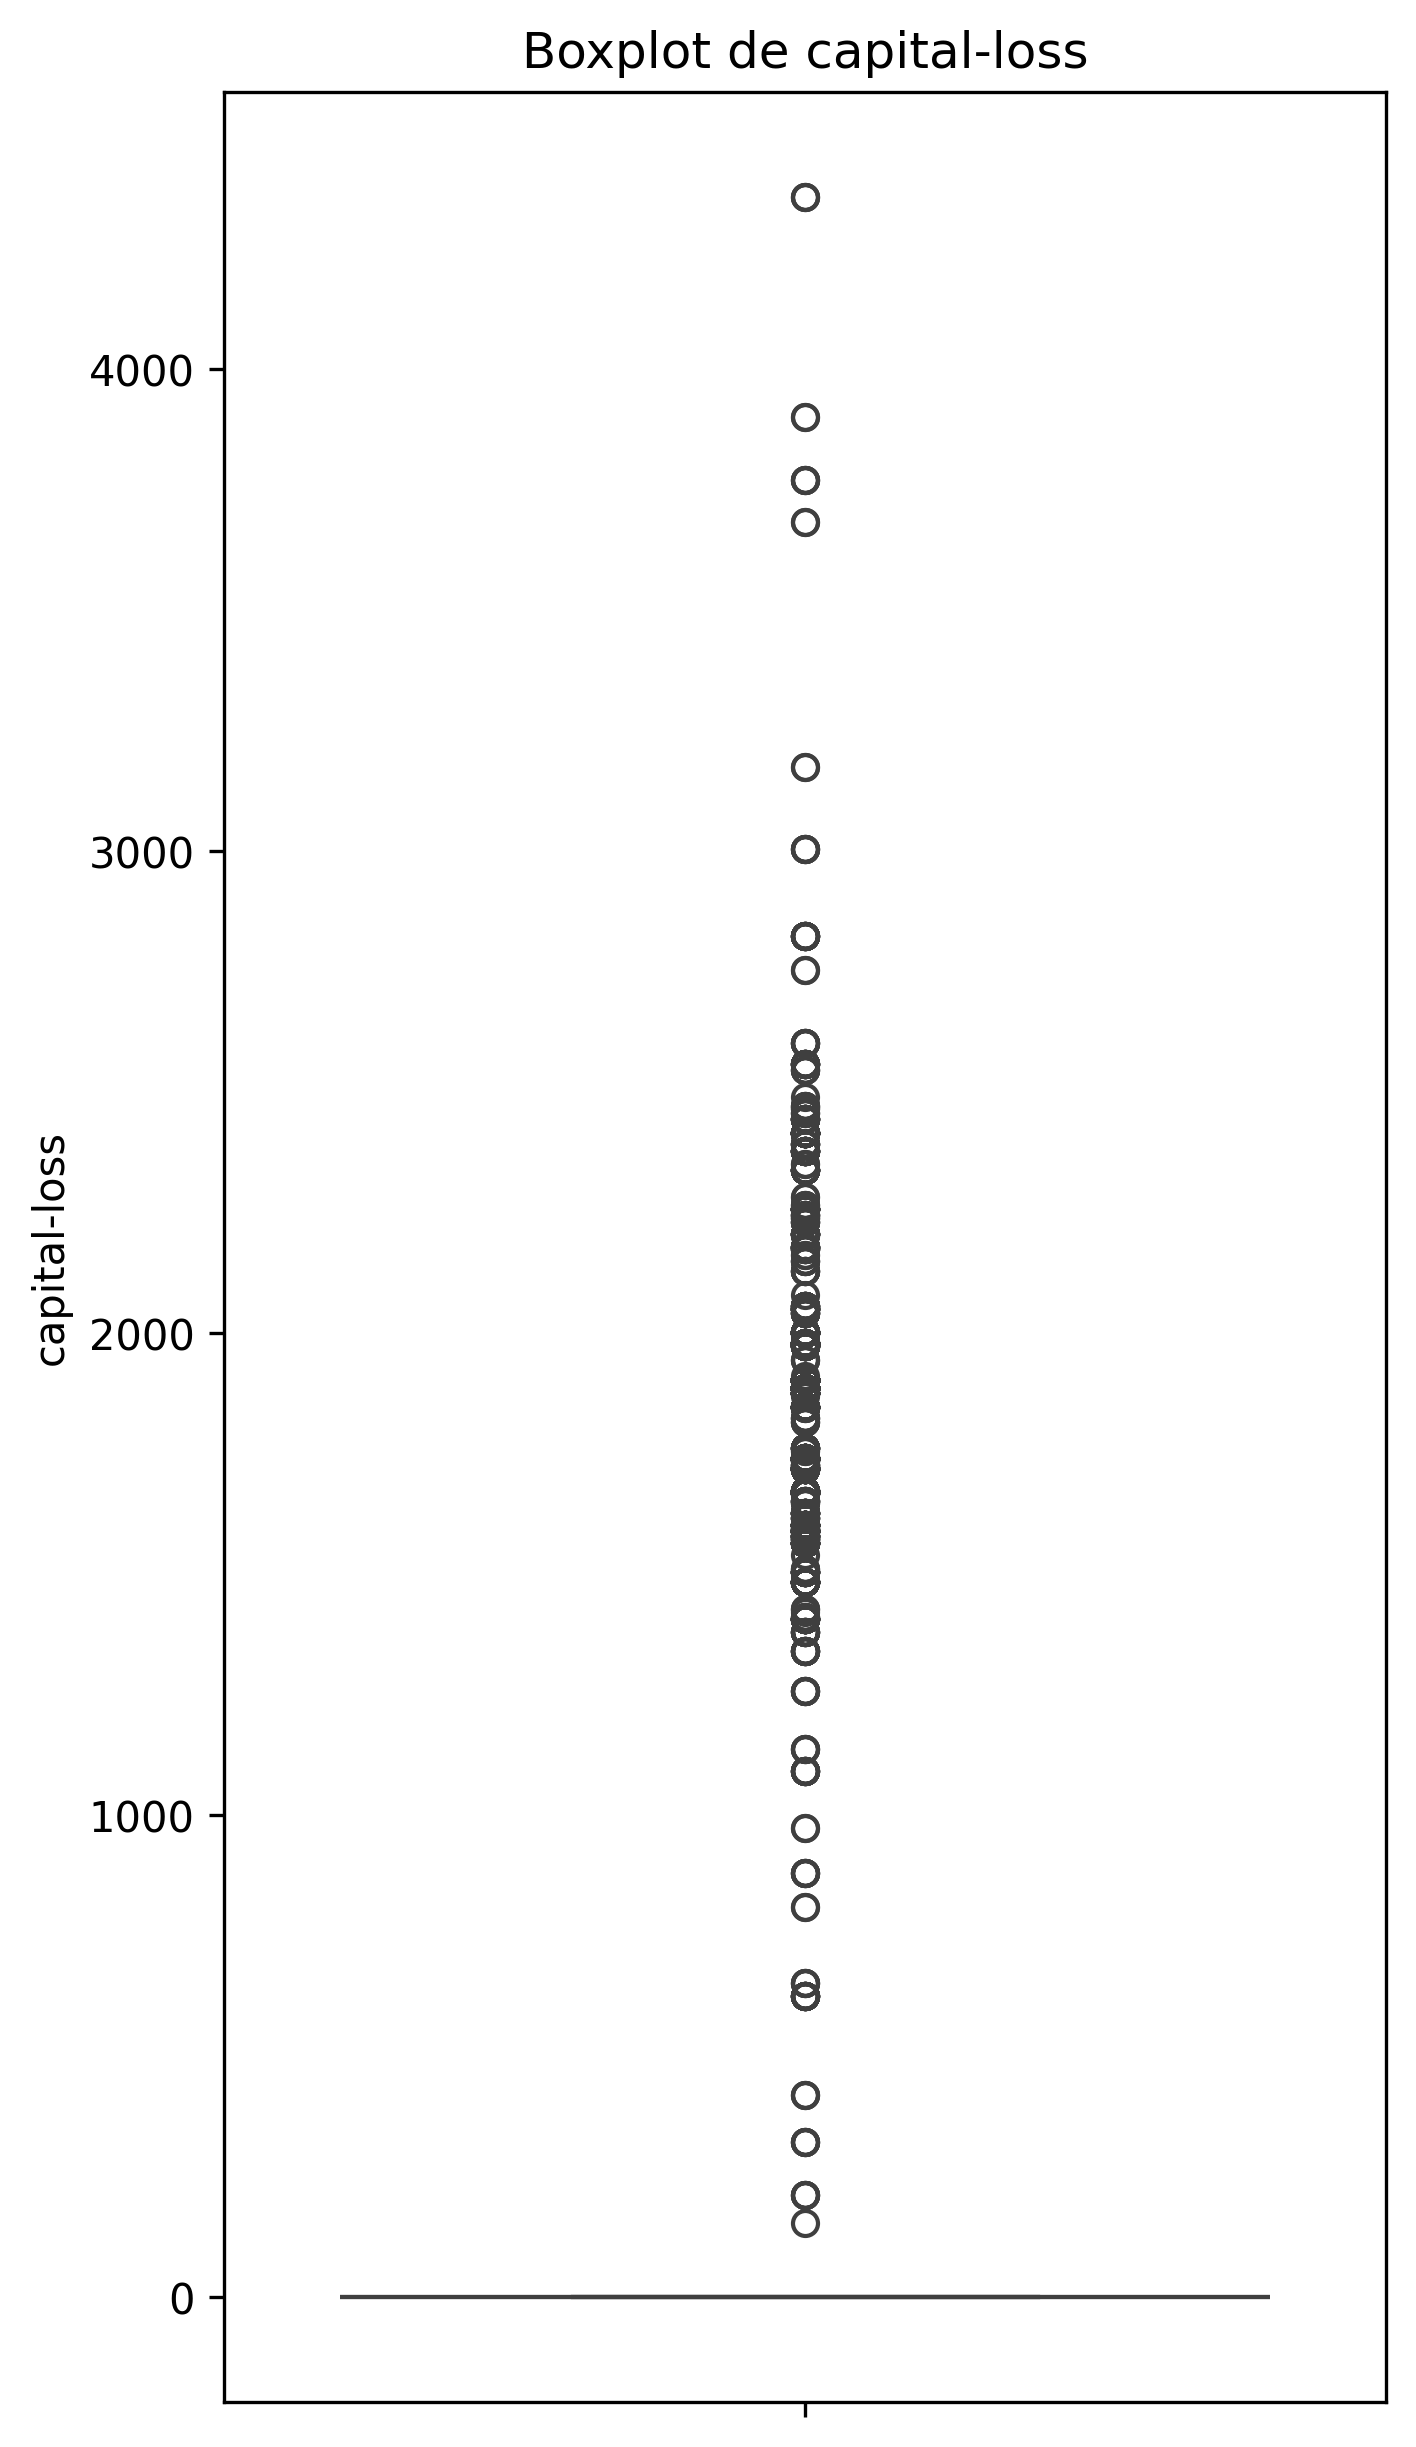
\includegraphics[width=\textwidth]{boxplot_capital-loss.png}
        \caption{Boxplot de \texttt{capital-loss}}
        \label{fig:capital_loss_boxplot}
      \end{subfigure}
      \caption{Distribución de \texttt{capital-loss}: histograma y boxplot.}
      \label{fig:capital_loss_visual}
    \end{figure}

    \emph{capital-loss} muestra un patrón similar al de \emph{capital-gain}: el 75\,\% de los registros 
    tienen valor cero y solo unos pocos presentan pérdidas elevadas. El boxplot evidencia que la mayor 
    variabilidad proviene de estos pocos casos extremos. Para facilitar el análisis, podría ser útil 
    transformar esta variable en binaria (pérdida sí/no) o aplicar técnicas que reduzcan el impacto de los 
    valores atípicos si se mantiene como variable continua.

    % Histograma y boxplot: education-num
    \begin{figure}[H]
      \centering
      \begin{subfigure}[b]{0.45\textwidth}
        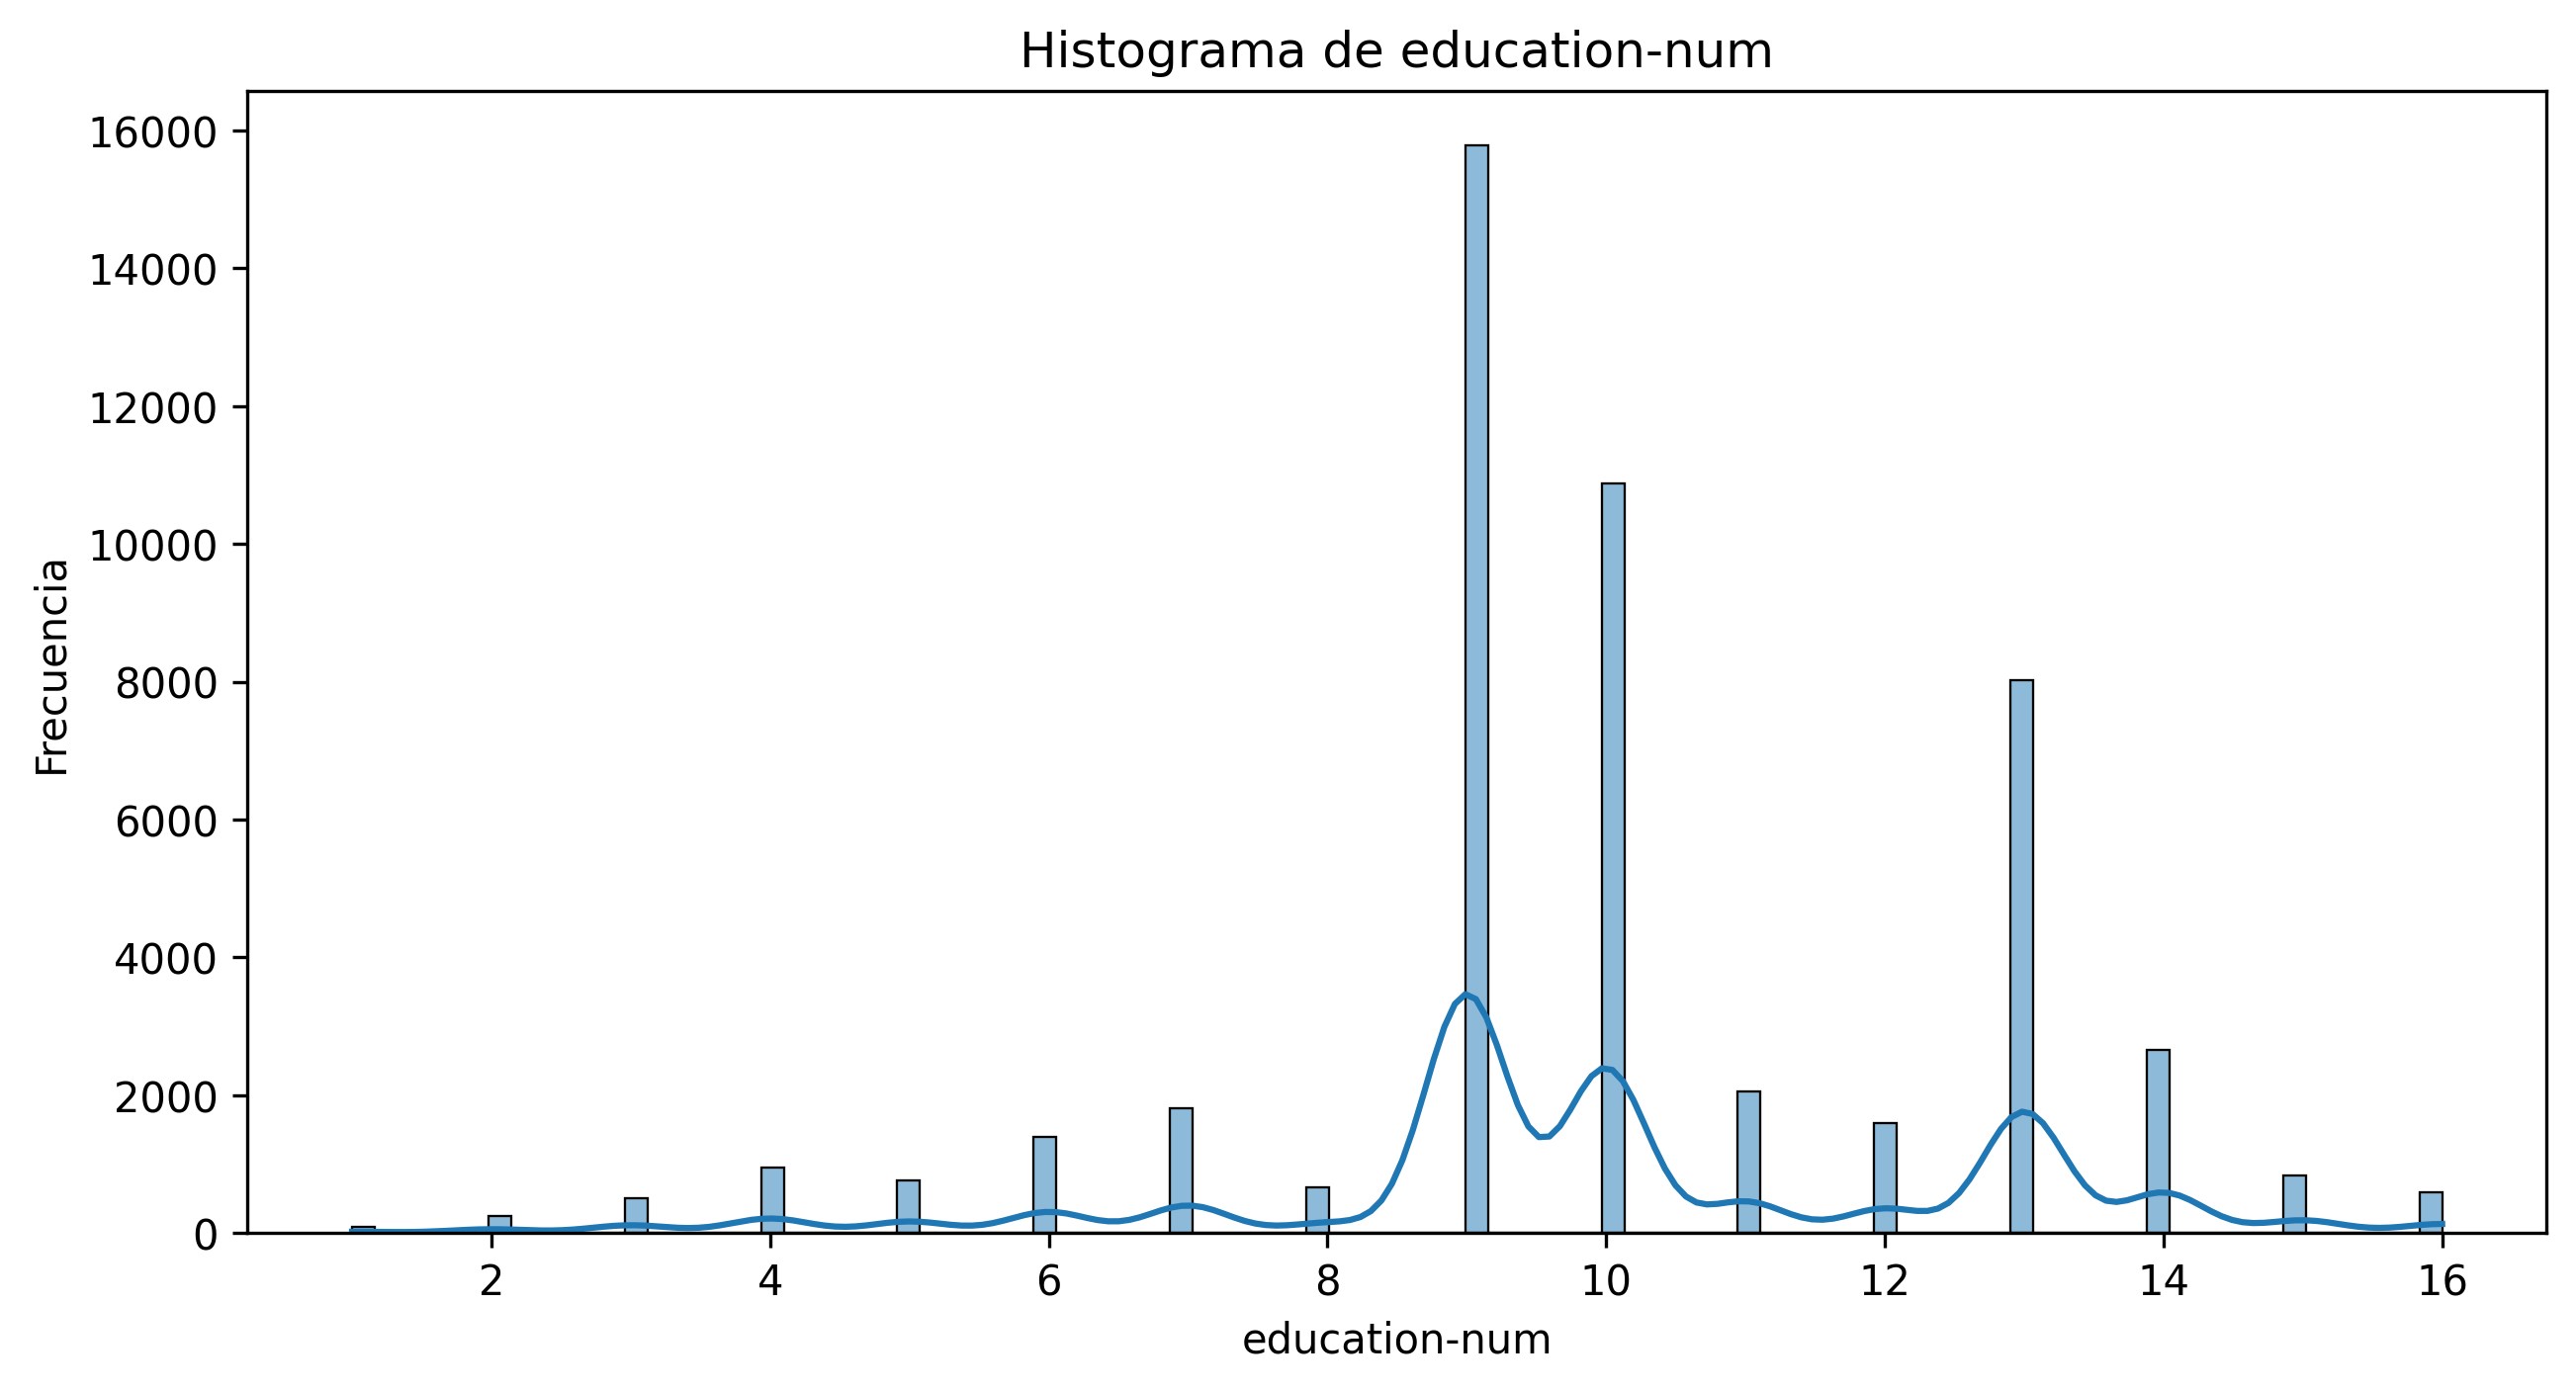
\includegraphics[width=\textwidth]{histogram_education-num.png}
        \caption{Histograma de \texttt{education-num}}
        \label{fig:education_num_hist}
      \end{subfigure}
      \hfill
      \begin{subfigure}[b]{0.45\textwidth}
        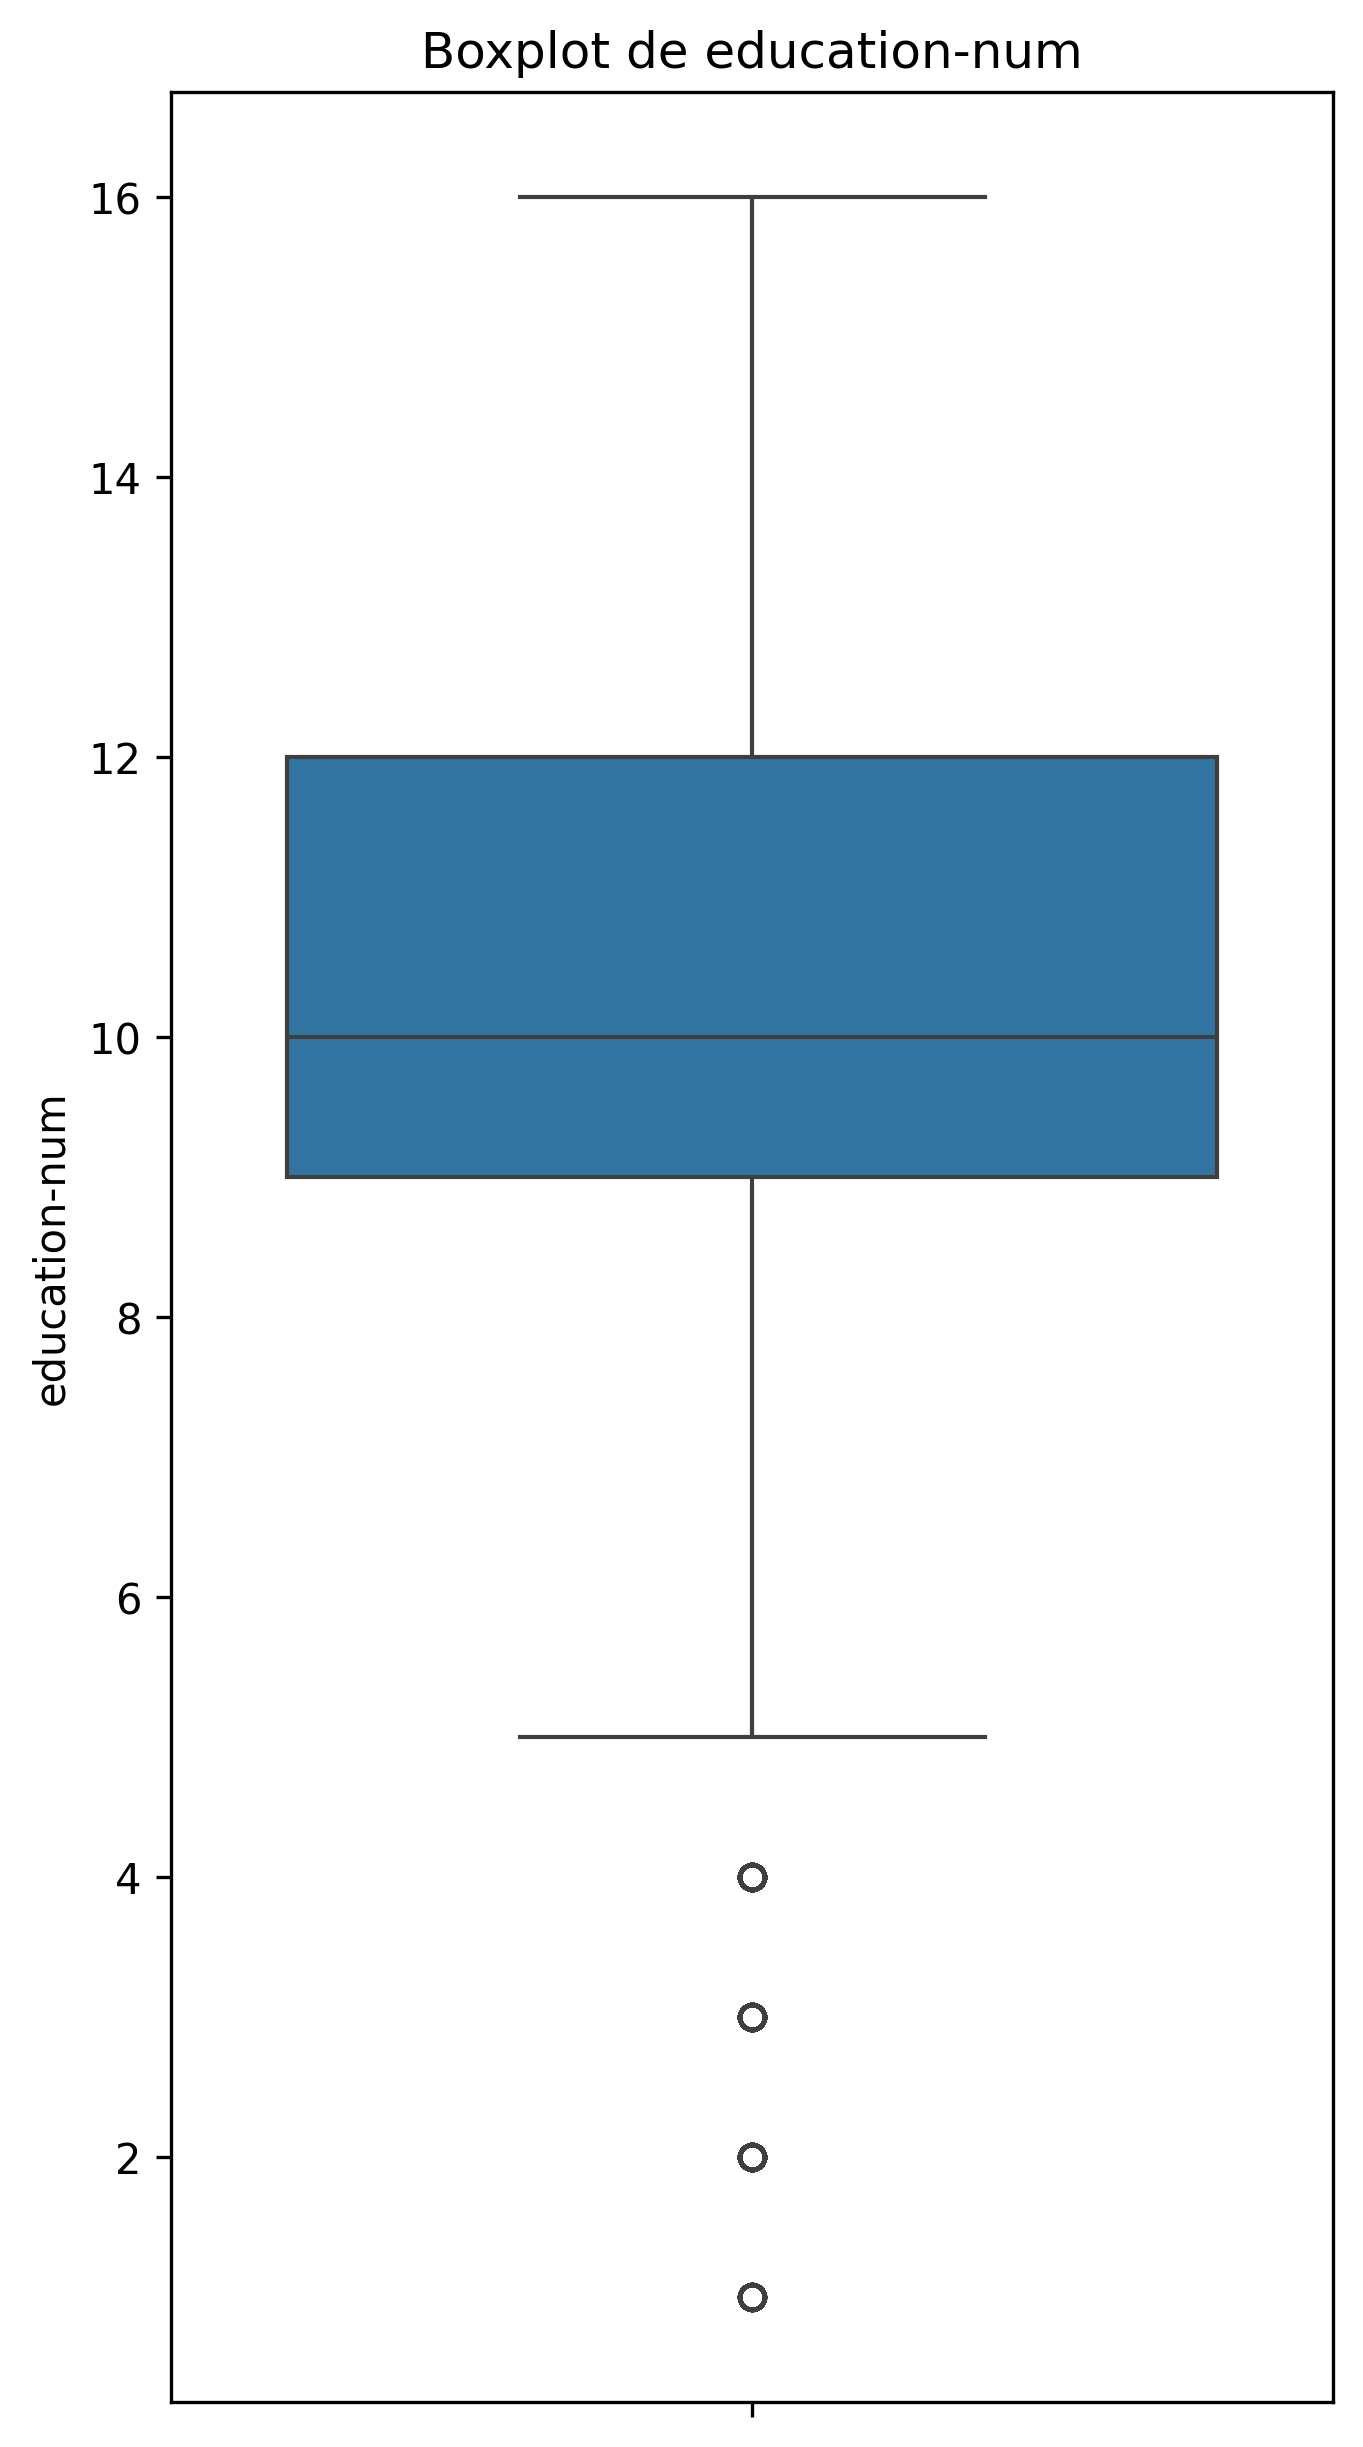
\includegraphics[width=\textwidth]{boxplot_education-num.png}
        \caption{Boxplot de \texttt{education-num}}
        \label{fig:education_num_boxplot}
      \end{subfigure}
      \caption{Distribución de \texttt{education-num}: histograma y boxplot.}
      \label{fig:education_num_visual}
    \end{figure}

    \emph{education-num} es una variable discreta entre 1 y 16, con mediana 10 y Q3=12. El histograma refleja picos en niveles 
    educativos frecuentes (por ejemplo, secundaria y algunos estudios superiores), y el boxplot confirma baja presencia de atípicos. 
    Su naturaleza ordinal sugiere que modelos lineales simples captan bien su efecto, aunque interacciones con \emph{hours-per-week} o 
    \emph{age} podrían aportar capacidad explicativa.

    % Histograma y boxplot: fnlwgt
    \begin{figure}[H]
      \centering
      \begin{subfigure}[b]{0.45\textwidth}
        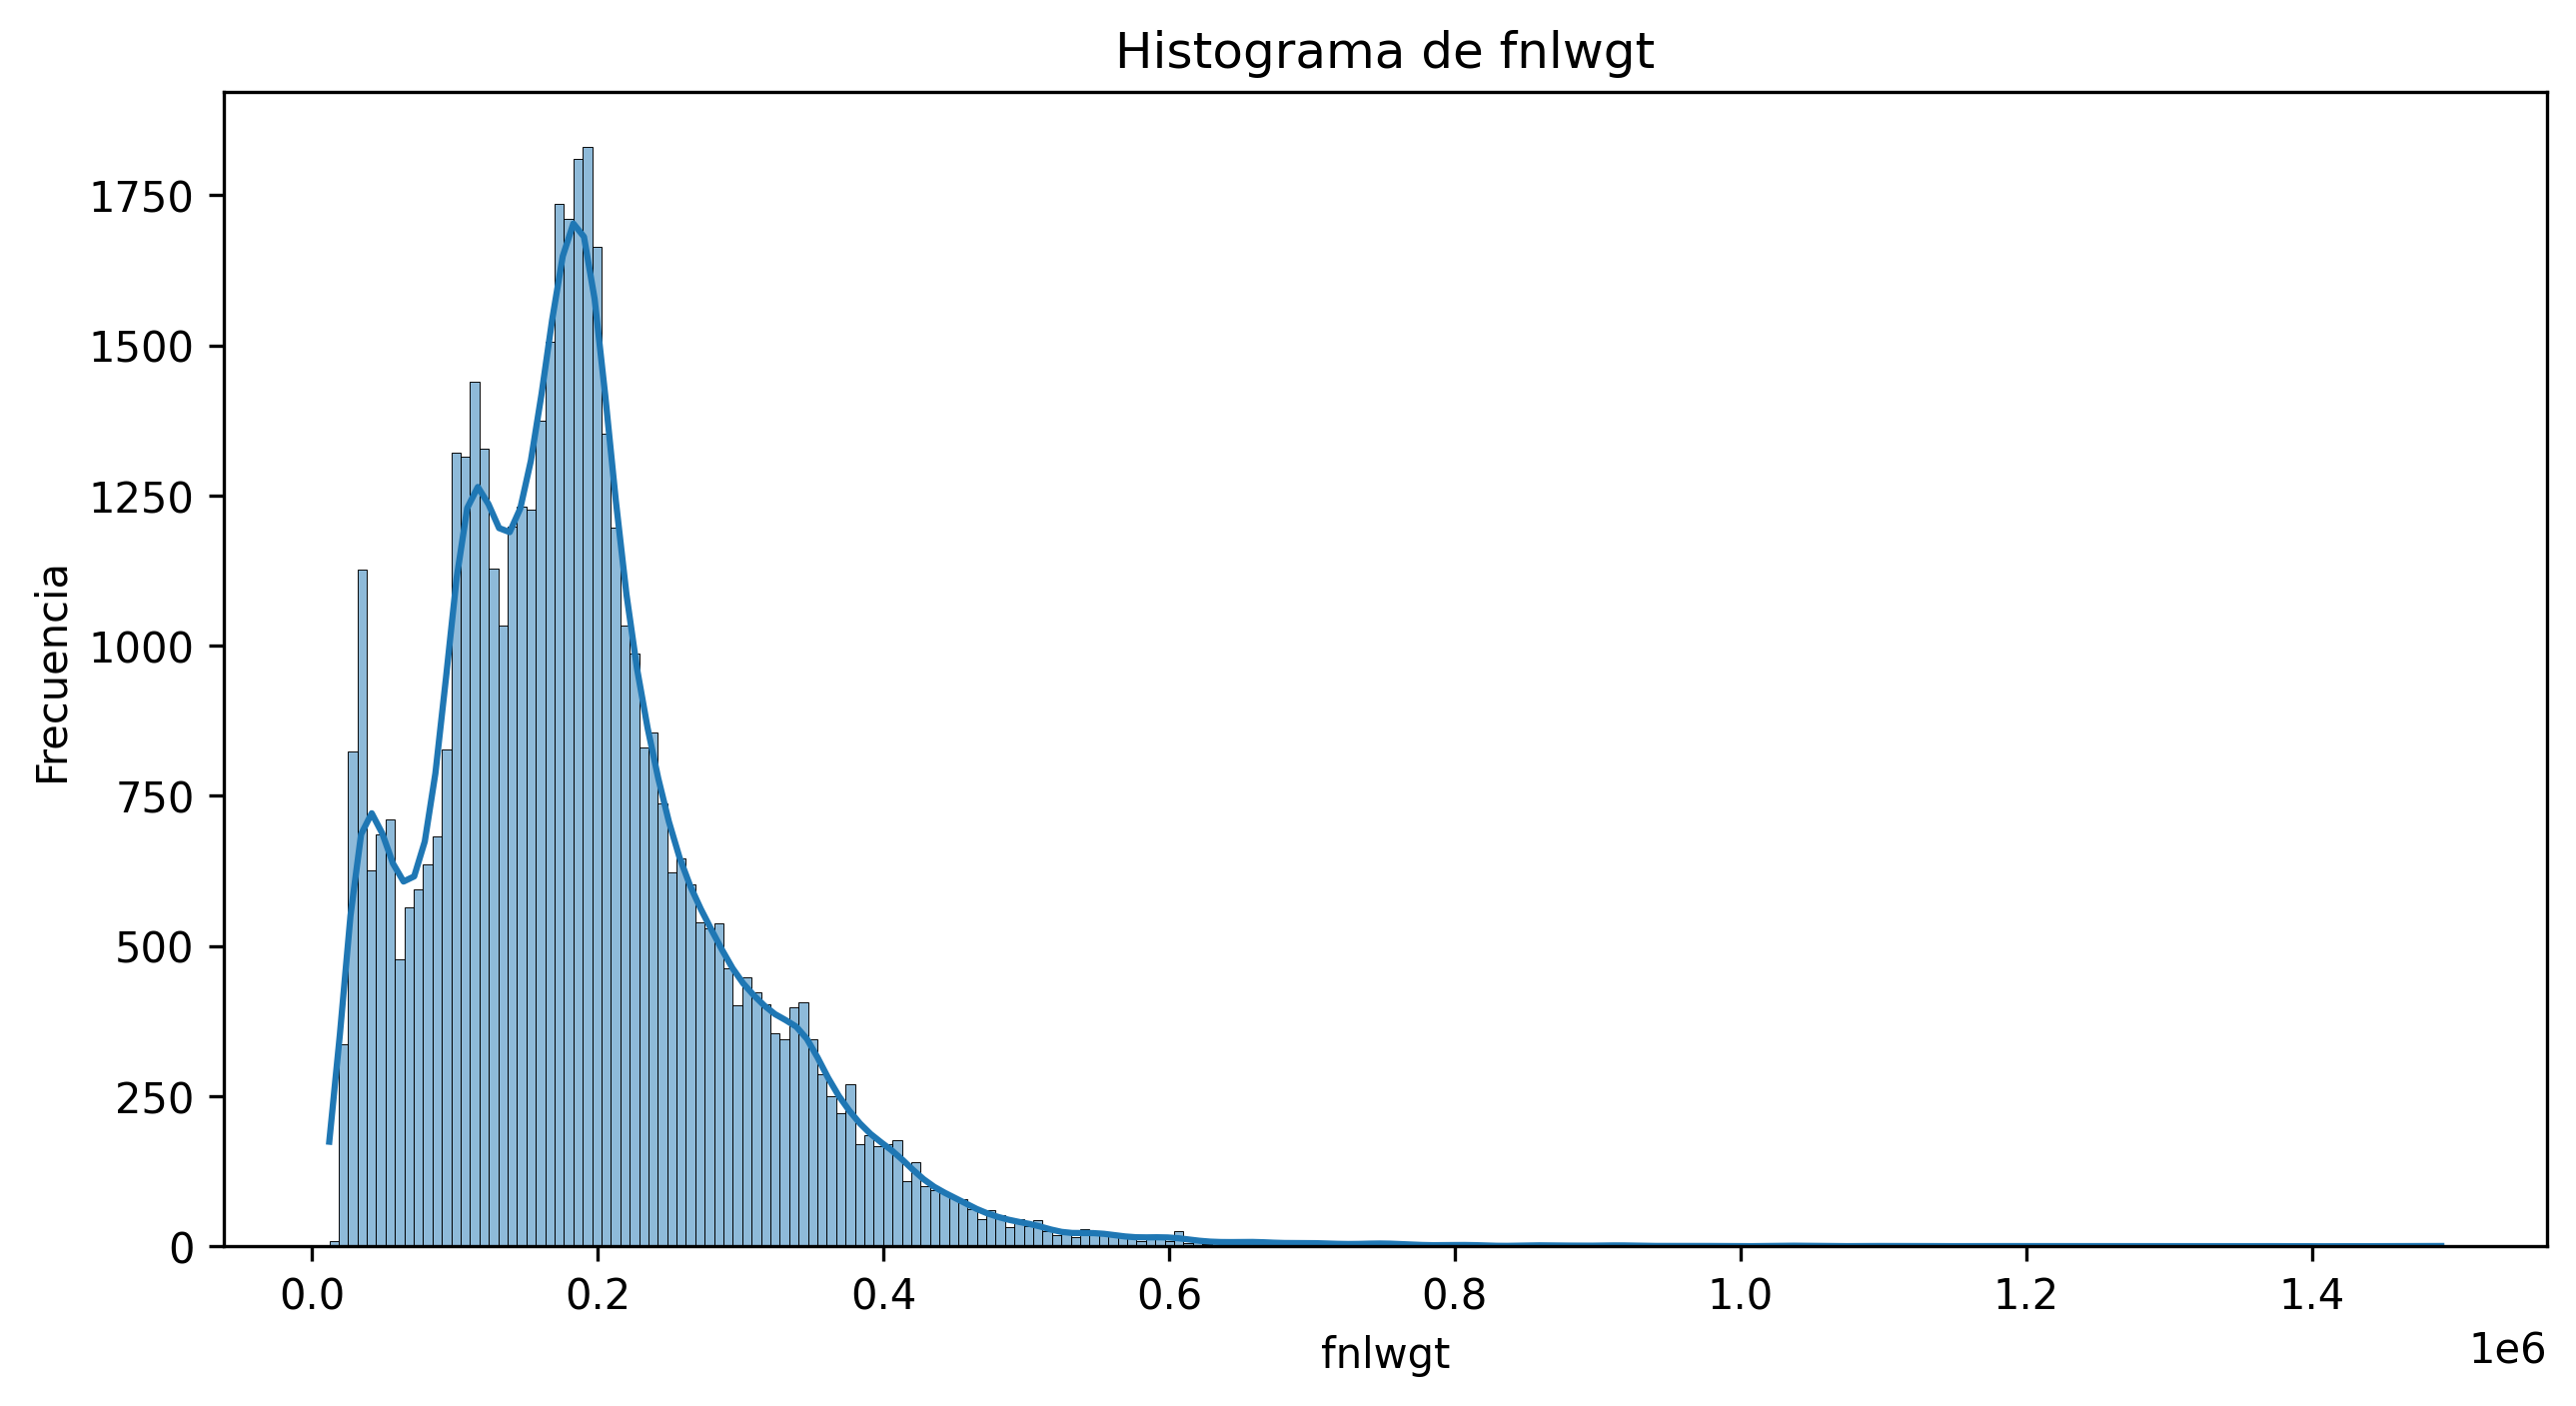
\includegraphics[width=\textwidth]{histogram_fnlwgt.png}
        \caption{Histograma de \texttt{fnlwgt}}
        \label{fig:fnlwgt_hist}
      \end{subfigure}
      \hfill
      \begin{subfigure}[b]{0.45\textwidth}
        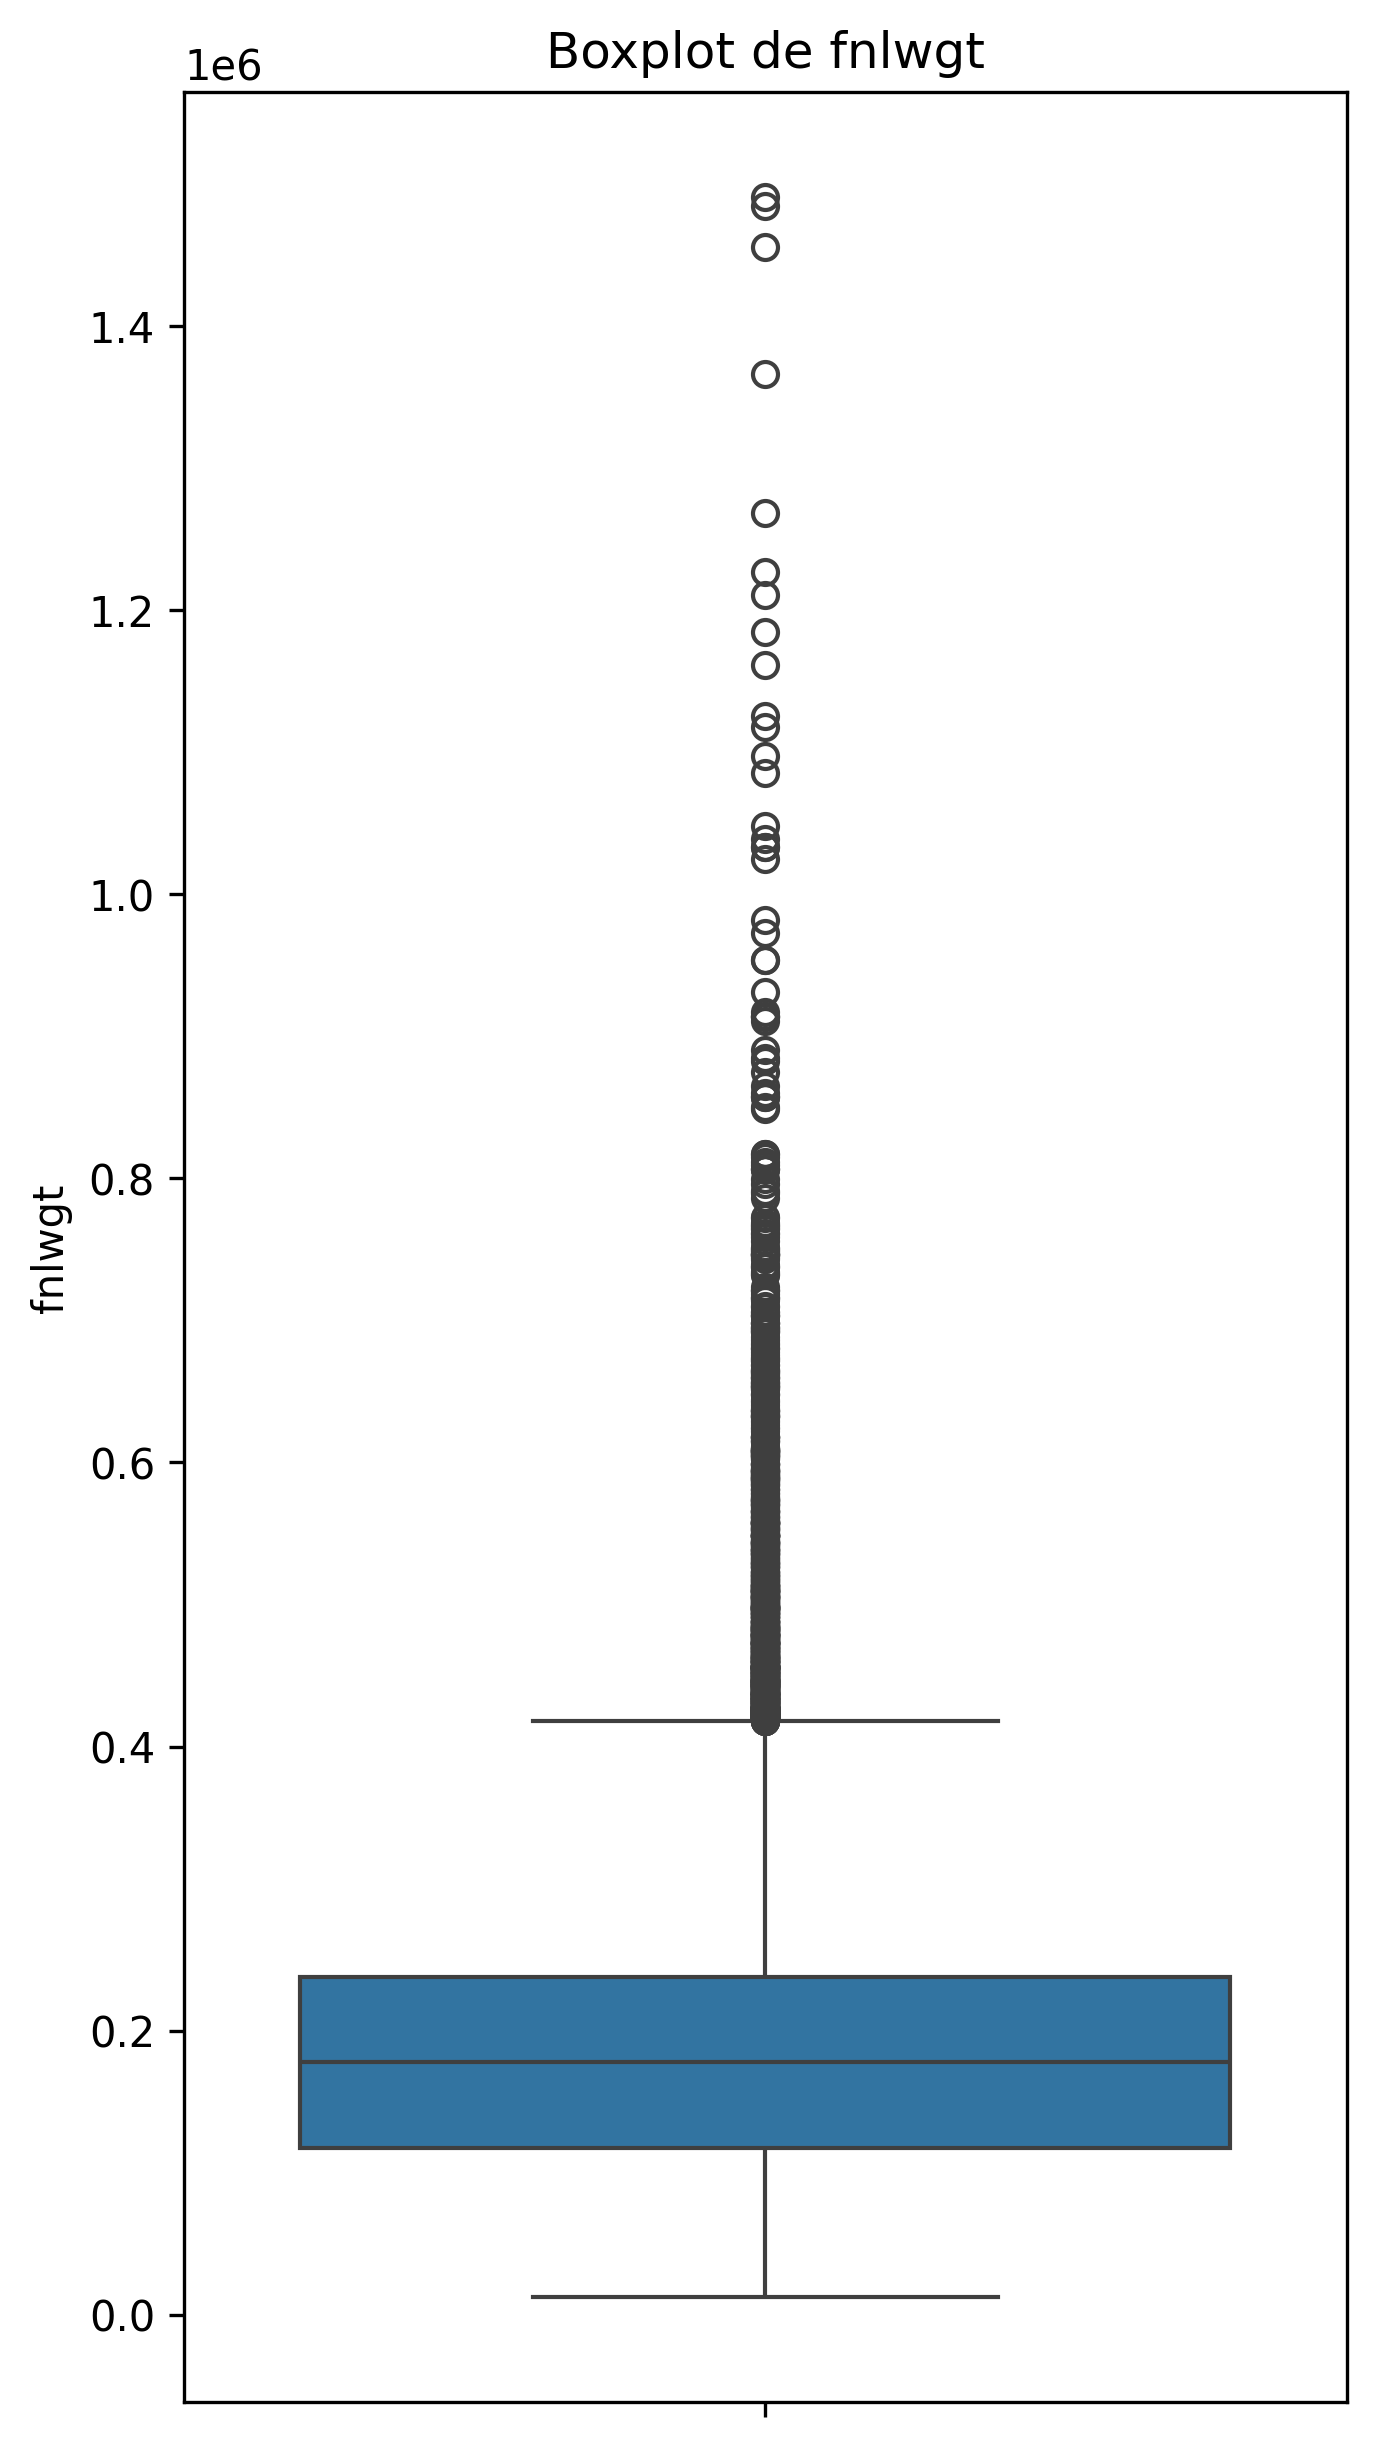
\includegraphics[width=\textwidth]{boxplot_fnlwgt.png}
        \caption{Boxplot de \texttt{fnlwgt}}
        \label{fig:fnlwgt_boxplot}
      \end{subfigure}
      \caption{Distribución de \texttt{fnlwgt}: histograma y boxplot.}
      \label{fig:fnlwgt_visual}
    \end{figure}

    \emph{fnlwgt} exhibe gran dispersión. El histograma muestra una cola derecha muy extensa y el boxplot múltiples valores atípicos altos. 
    Si se utiliza como predictor, convendría probar transformaciones logarítmicas o normalizaciones robustas.

    % Histograma y boxplot: hours-per-week
    \begin{figure}[H]
      \centering
      \begin{subfigure}[b]{0.45\textwidth}
        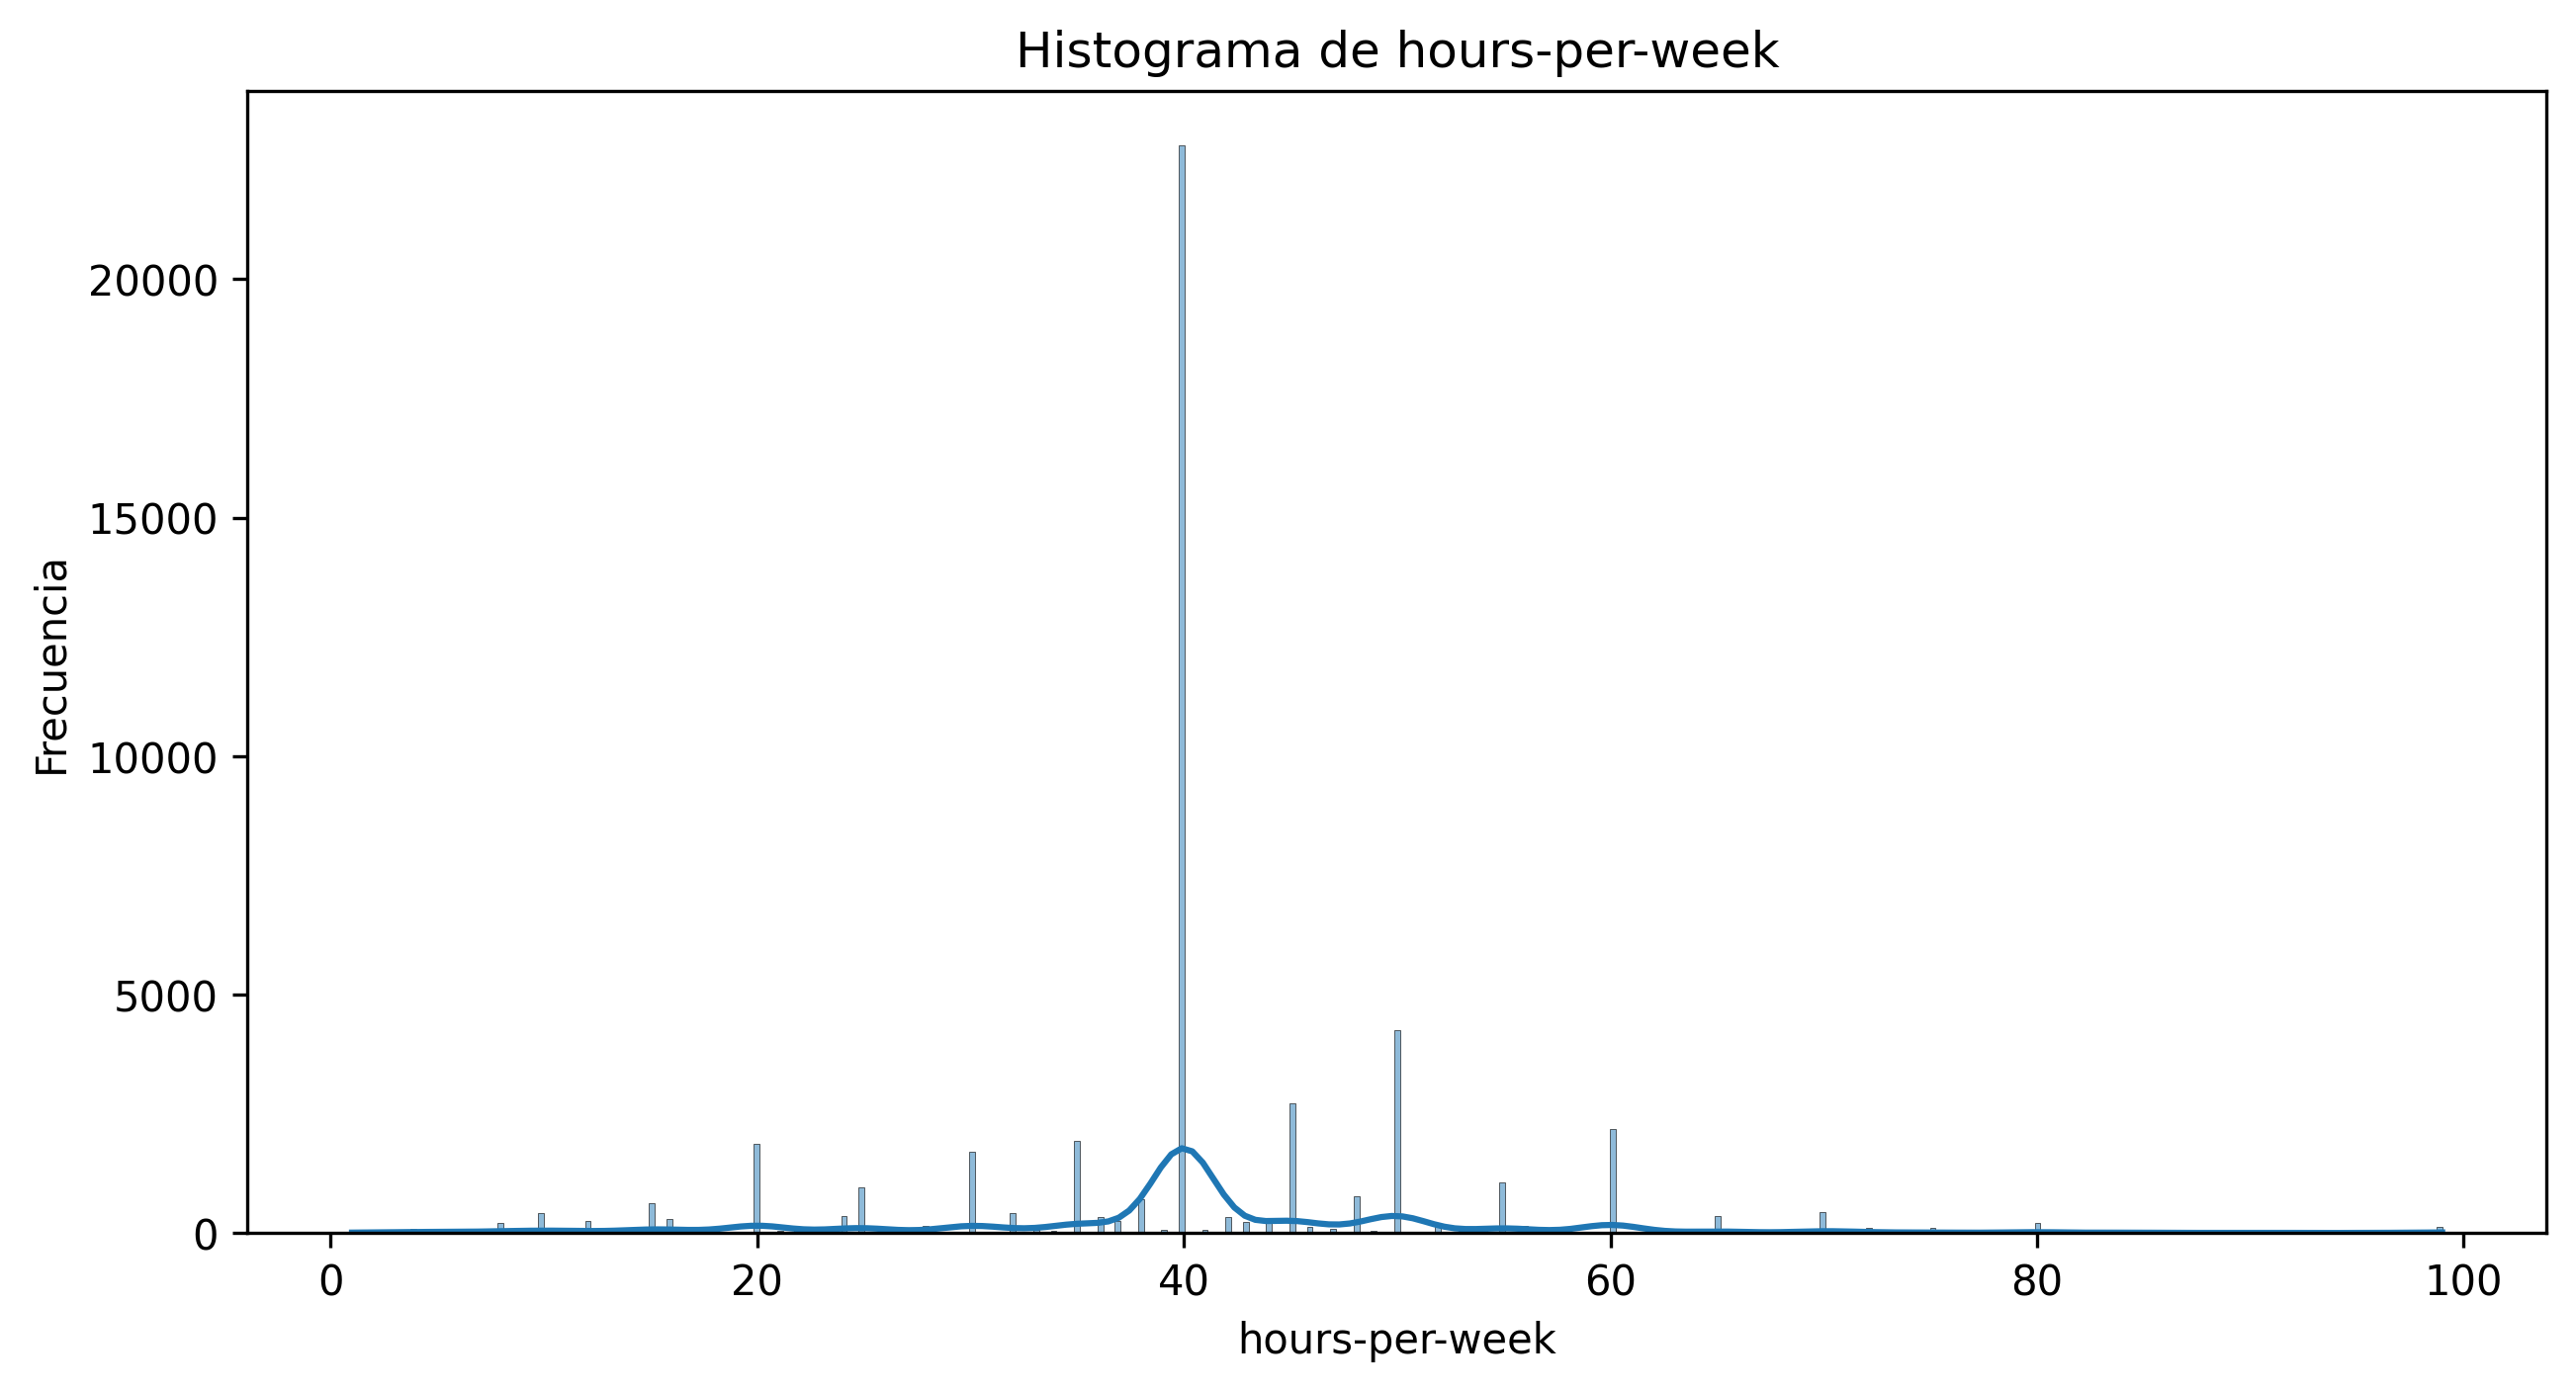
\includegraphics[width=\textwidth]{histogram_hours-per-week.png}
        \caption{Histograma de \texttt{hours-per-week}}
        \label{fig:hours_per_week_hist}
      \end{subfigure}
      \hfill
      \begin{subfigure}[b]{0.45\textwidth}
        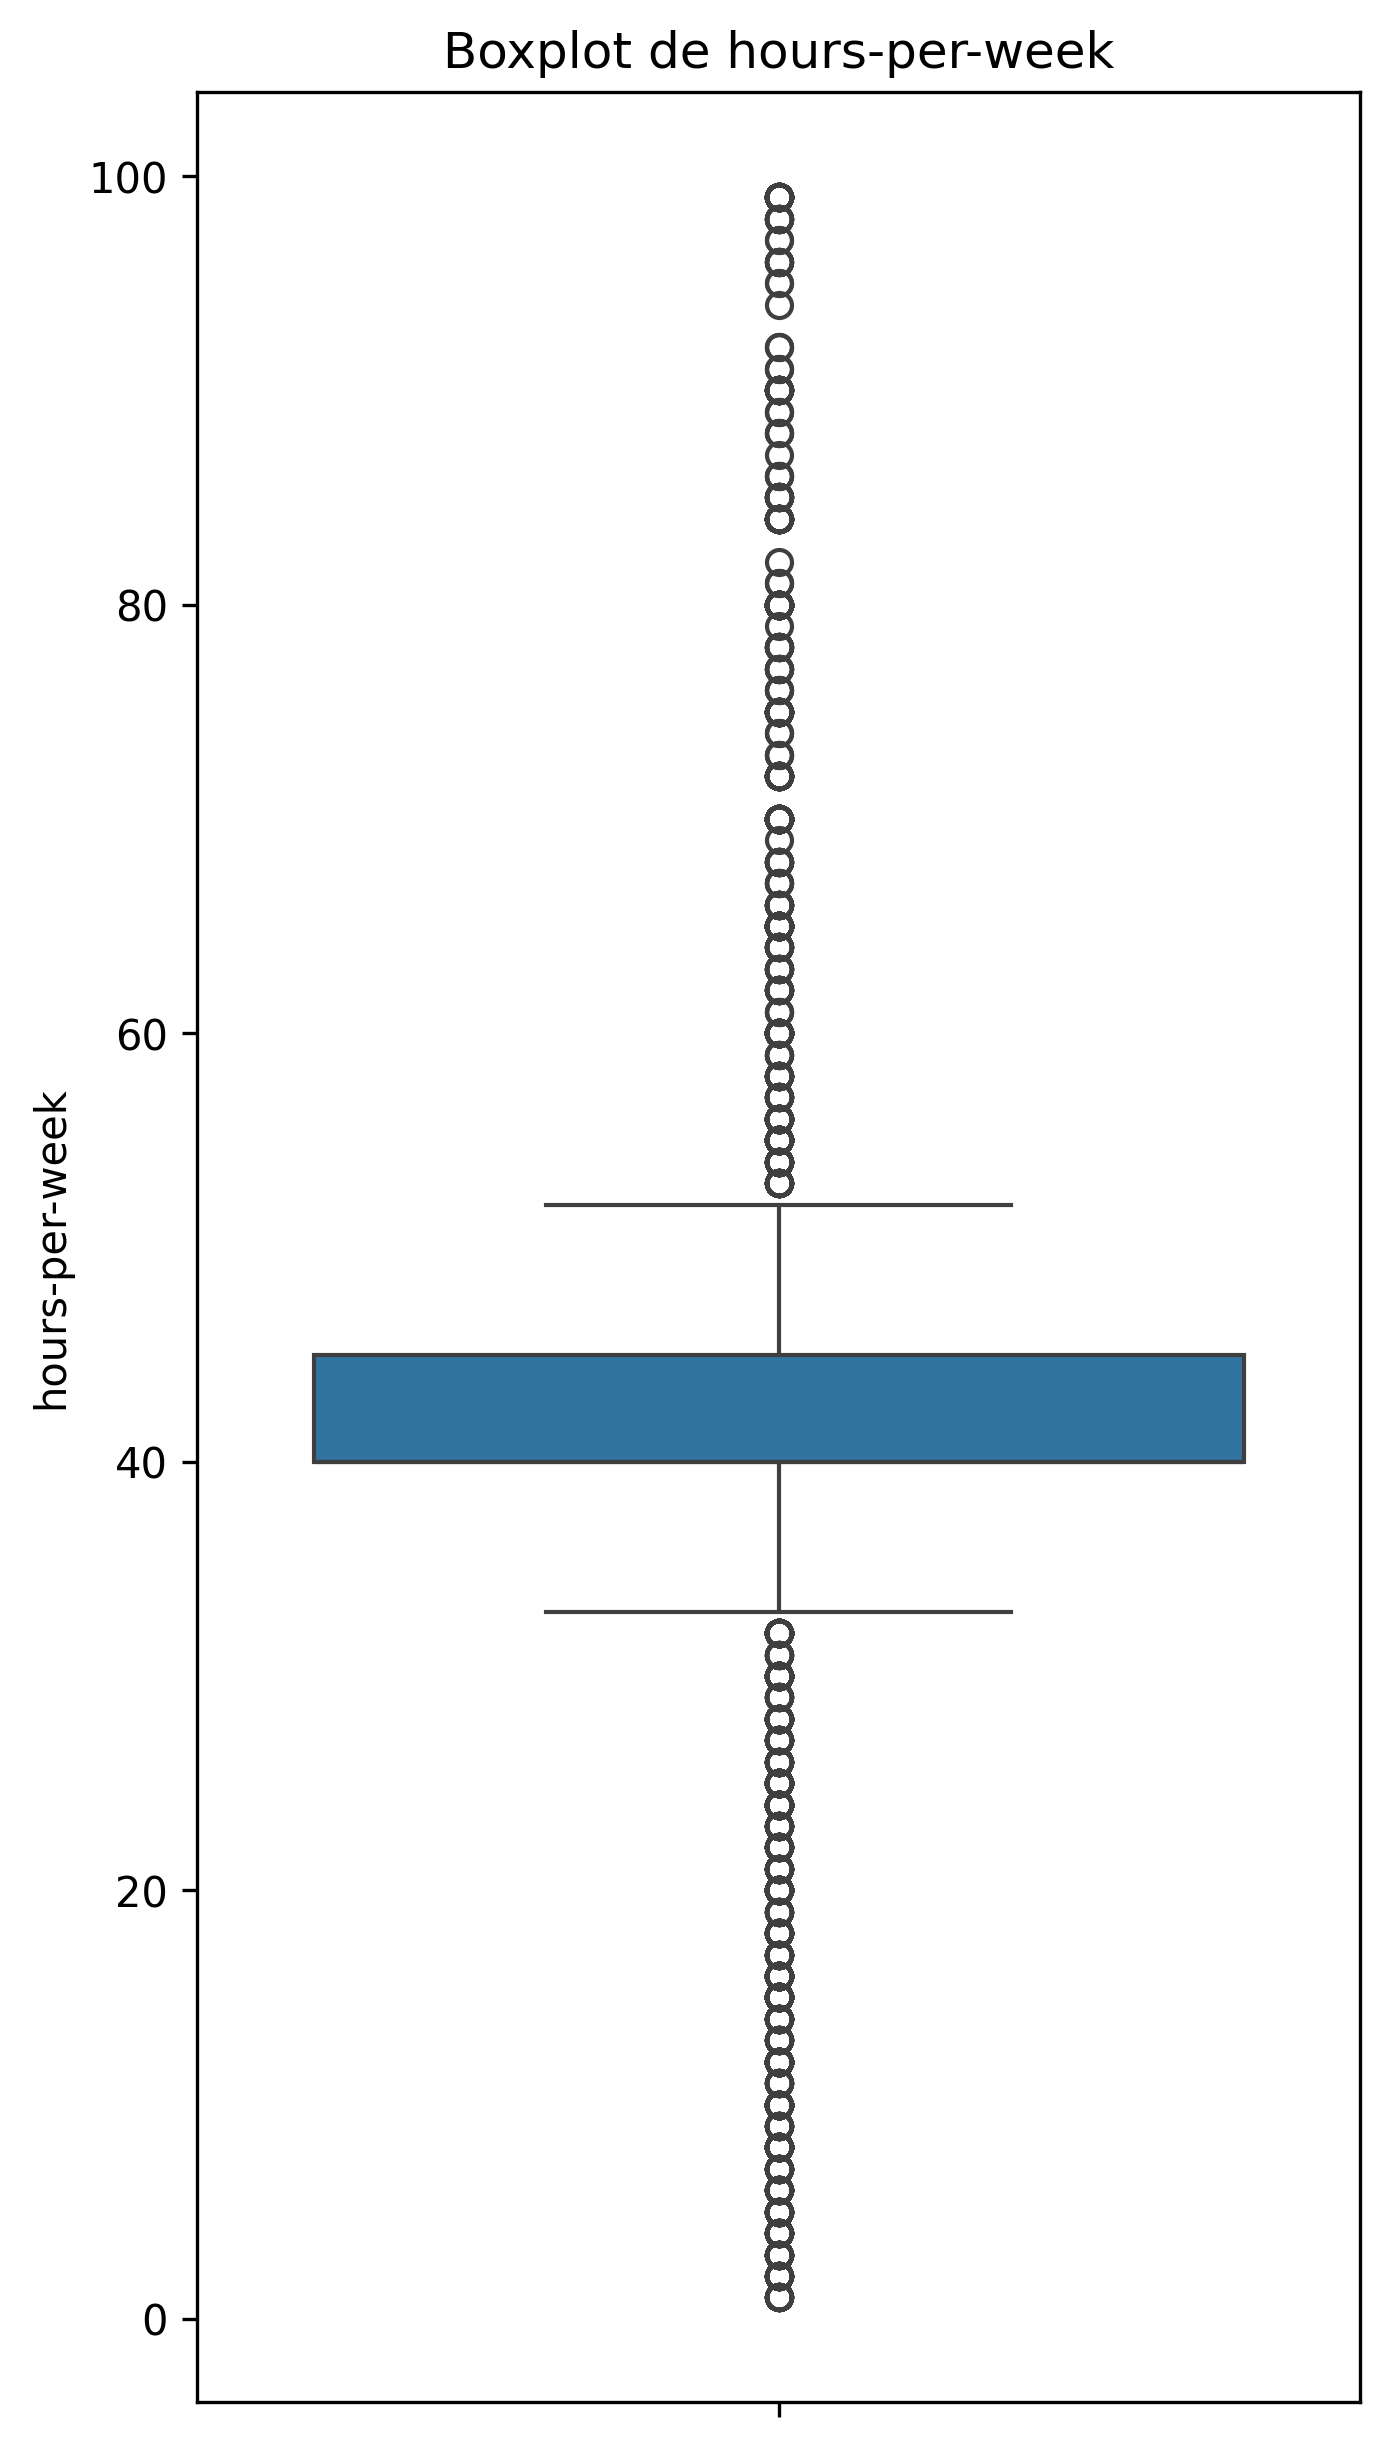
\includegraphics[width=\textwidth]{boxplot_hours-per-week.png}
        \caption{Boxplot de \texttt{hours-per-week}}
        \label{fig:hours_per_week_boxplot}
      \end{subfigure}
      \caption{Distribución de \texttt{hours-per-week}: histograma y boxplot.}
      \label{fig:hours_per_week_visual}
    \end{figure}

    La jornada semanal se concentra en 40 horas (mediana=40), con un incremento hacia 45 horas en Q3 y una cola derecha moderada hasta 99. 
    El histograma sugiere picos en 40 y 45, lo que es esperado si se supone que las personas trabajan 8 horas durante 5 días. El boxplot indica 
    pocos valores atípicos altos.

    % Histograma variable objetivo (income)
    \begin{figure}[H]
      \centering
      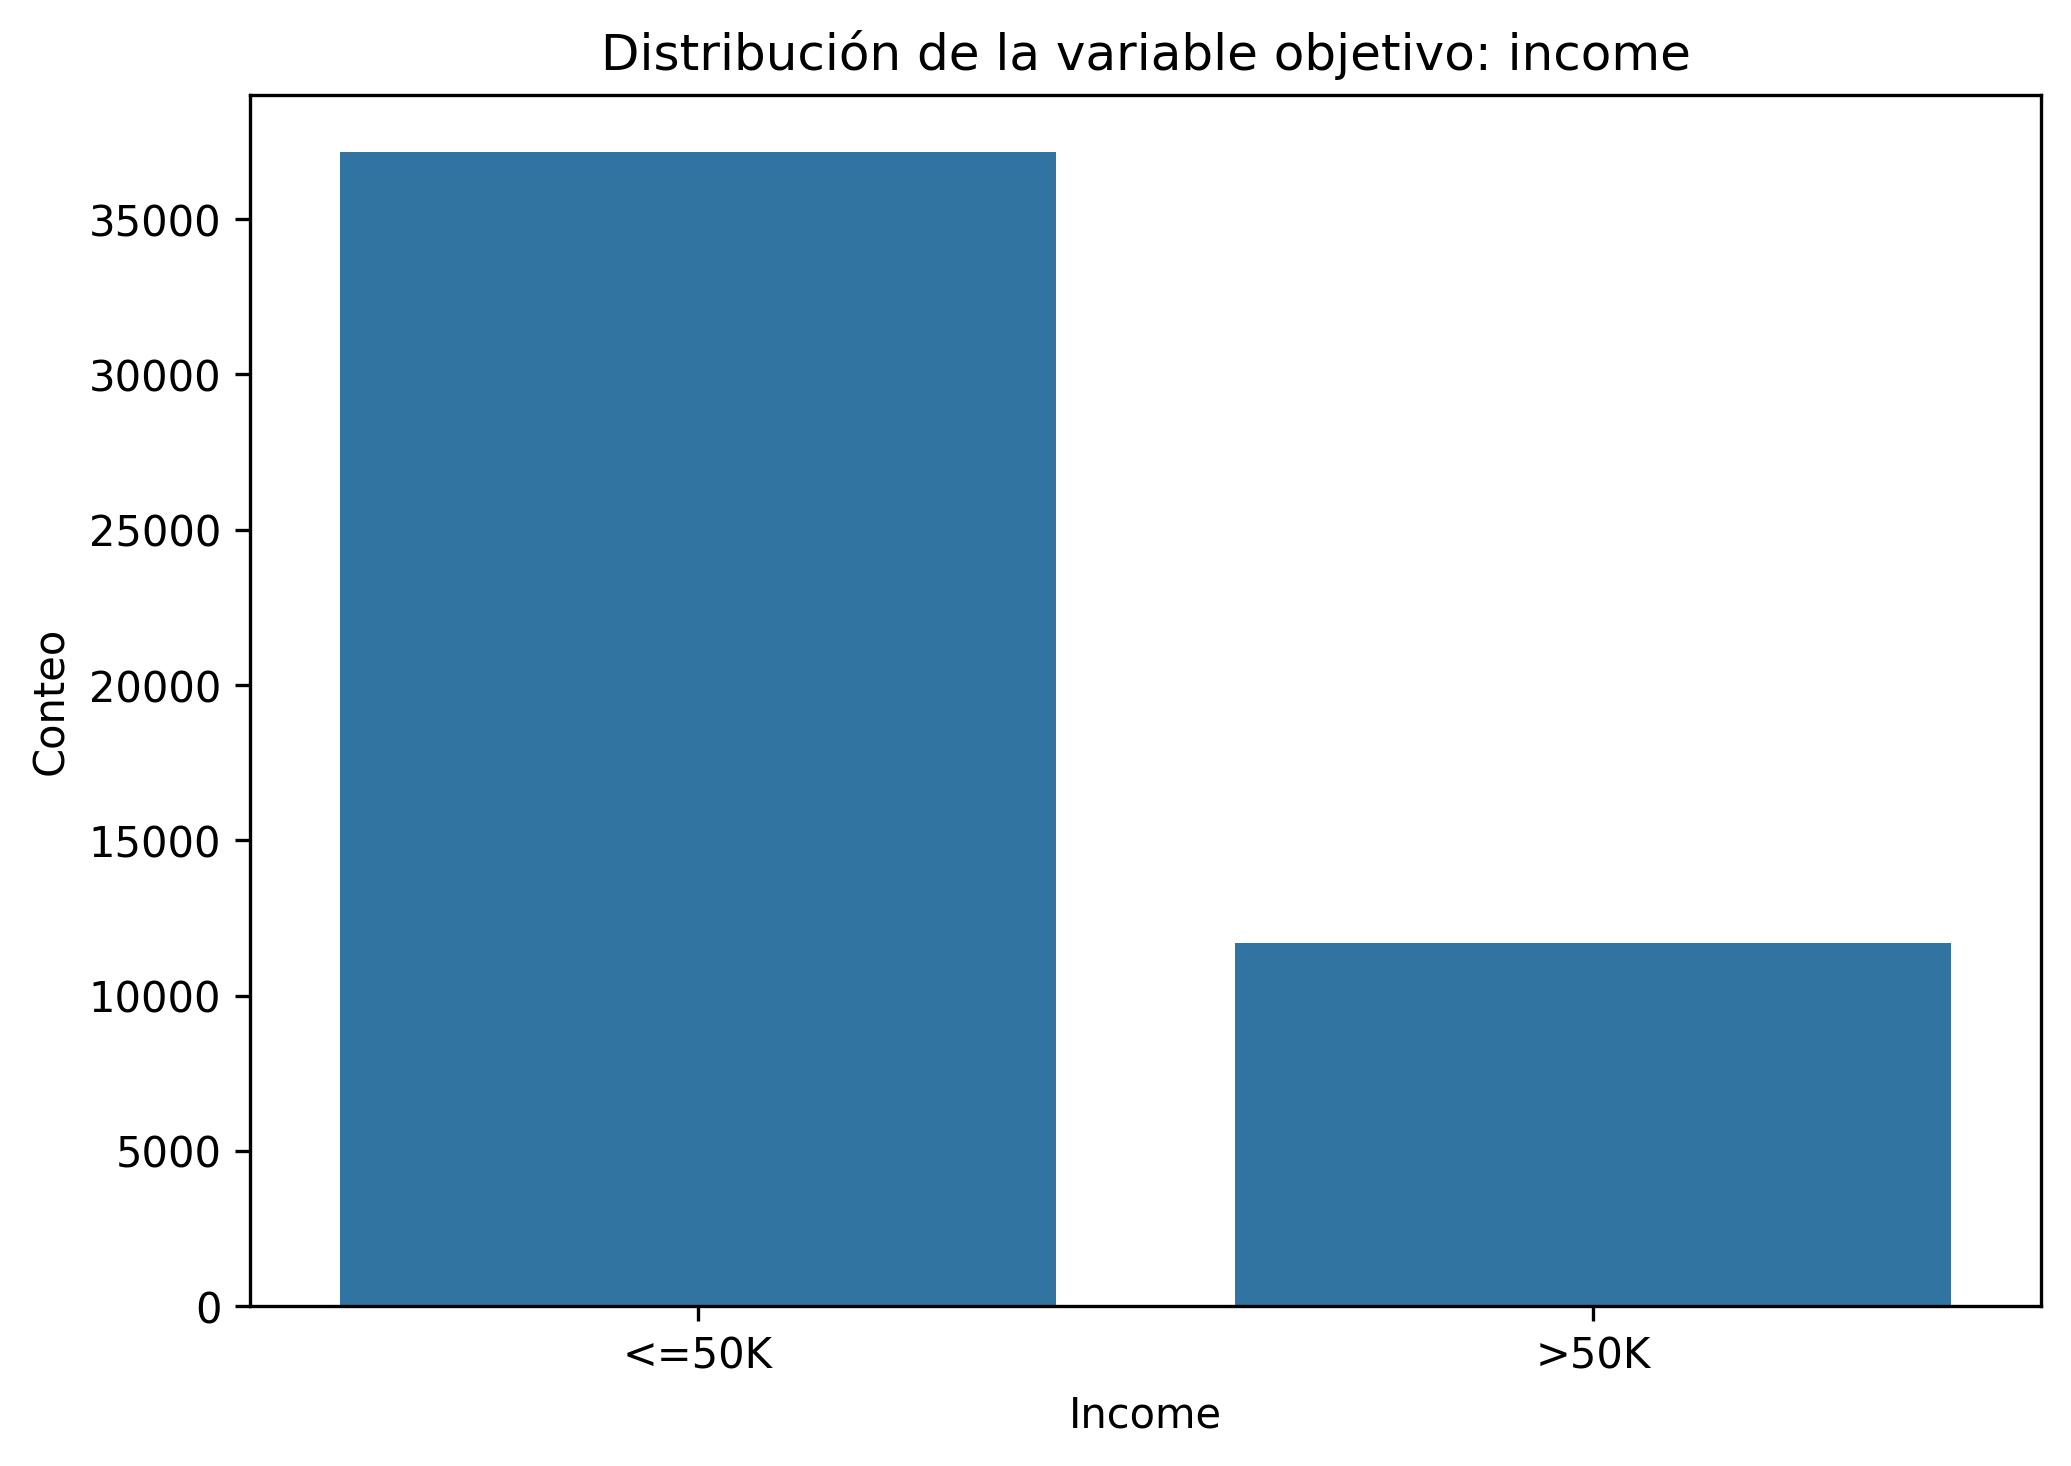
\includegraphics[width=0.6\textwidth]{income_distribution.png}
      \caption{Histograma de la variable objetivo \texttt{income}.}
      \label{fig:income_hist}
    \end{figure}

    La \Cref{fig:income_hist} muestra un claro desequilibrio a favor de la categoría \texttt{<=50K}, lo cual puede afectar el desempeño de 
    los modelos de clasificación.

    \item \textbf{Q2: Limpieza y preprocesamiento de datos}
    \begin{itemize}
      \item \textbf{Valores nulos.} No se encontraron valores faltantes.
      
      \begin{table}[H]
        \centering
        \begin{tabular}{@{}lcc@{}}
          \toprule
          \textbf{Columna} & \textbf{Nulos (conteo)} & \textbf{Nulos (\%)} \\
          \midrule
          age & 0 & 0.0 \\ workclass & 0 & 0.0 \\ fnlwgt & 0 & 0.0 \\ education & 0 & 0.0 \\
          education-num & 0 & 0.0 \\ marital-status & 0 & 0.0 \\ occupation & 0 & 0.0 \\
          relationship & 0 & 0.0 \\ race & 0 & 0.0 \\ sex & 0 & 0.0 \\
          capital-gain & 0 & 0.0 \\ capital-loss & 0 & 0.0 \\ hours-per-week & 0 & 0.0 \\
          native-country & 0 & 0.0 \\ income & 0 & 0.0 \\
          \bottomrule
        \end{tabular}
        \caption{Conteo y porcentaje de valores nulos por columna.}
        \label{tab:null_values}
      \end{table}

      \item \textbf{Duplicados.} Se identificaron 29 filas duplicadas y se eliminaron. No obstante, podrían corresponder a personas 
      distintas con la misma combinación de atributos.

      \item \textbf{Tratamiento de faltantes.} Al no haber valores nulos, no fue necesaria la imputación ni eliminación adicional.
    \end{itemize}

    \item \textbf{Q3: División del dataset}
    \begin{itemize}
      \item \textbf{Split 80/20.} Se dividió en entrenamiento (80\,\%) y prueba (20\,\%) preservando la proporción de \texttt{income}.
      \item \textbf{Balance por clase.} La \Cref{tab:income_proportion} muestra que la proporción por clase es prácticamente idéntica en ambos conjuntos.

      \begin{table}[H]
        \centering
        \sisetup{round-mode=places, round-precision=6}
        \begin{tabular}{@{}lS[table-format=1.6]S[table-format=1.6]@{}}
          \toprule
          \textbf{Categoría (\texttt{income})} & \textbf{Entrenamiento} & \textbf{Prueba} \\
          \midrule
          \texttt{<=50K} & 0.760581 & 0.760607 \\
          \texttt{>50K}  & 0.239419 & 0.239393 \\
          \bottomrule
        \end{tabular}
        \caption{Proporción de \texttt{income} en entrenamiento y prueba.}
        \label{tab:income_proportion}
      \end{table}

      \item \textbf{Tamaños de los conjuntos.}
      \begin{table}[H]
        \centering
        \begin{tabular}{@{}lll@{}}
          \toprule
          \textbf{Conjunto} & \textbf{Forma} & \textbf{Descripción} \\
          \midrule
          \texttt{X\_train} & (39032, 14) & Características de entrenamiento \\
          \texttt{X\_test}  & (9758, 14)  & Características de prueba \\
          \texttt{y\_train} & (39032,)    & Etiquetas de entrenamiento \\
          \texttt{y\_test}  & (9758,)     & Etiquetas de prueba \\
          \bottomrule
        \end{tabular}
        \caption{Tamaños de los conjuntos de entrenamiento y prueba.}
        \label{tab:train_test_shapes}
      \end{table}
    \end{itemize}

    \item \textbf{Q4: Correlaciones y relaciones}
    \begin{itemize}
      \item \textbf{Matriz de correlación.}
      \begin{figure}[H]
        \centering
        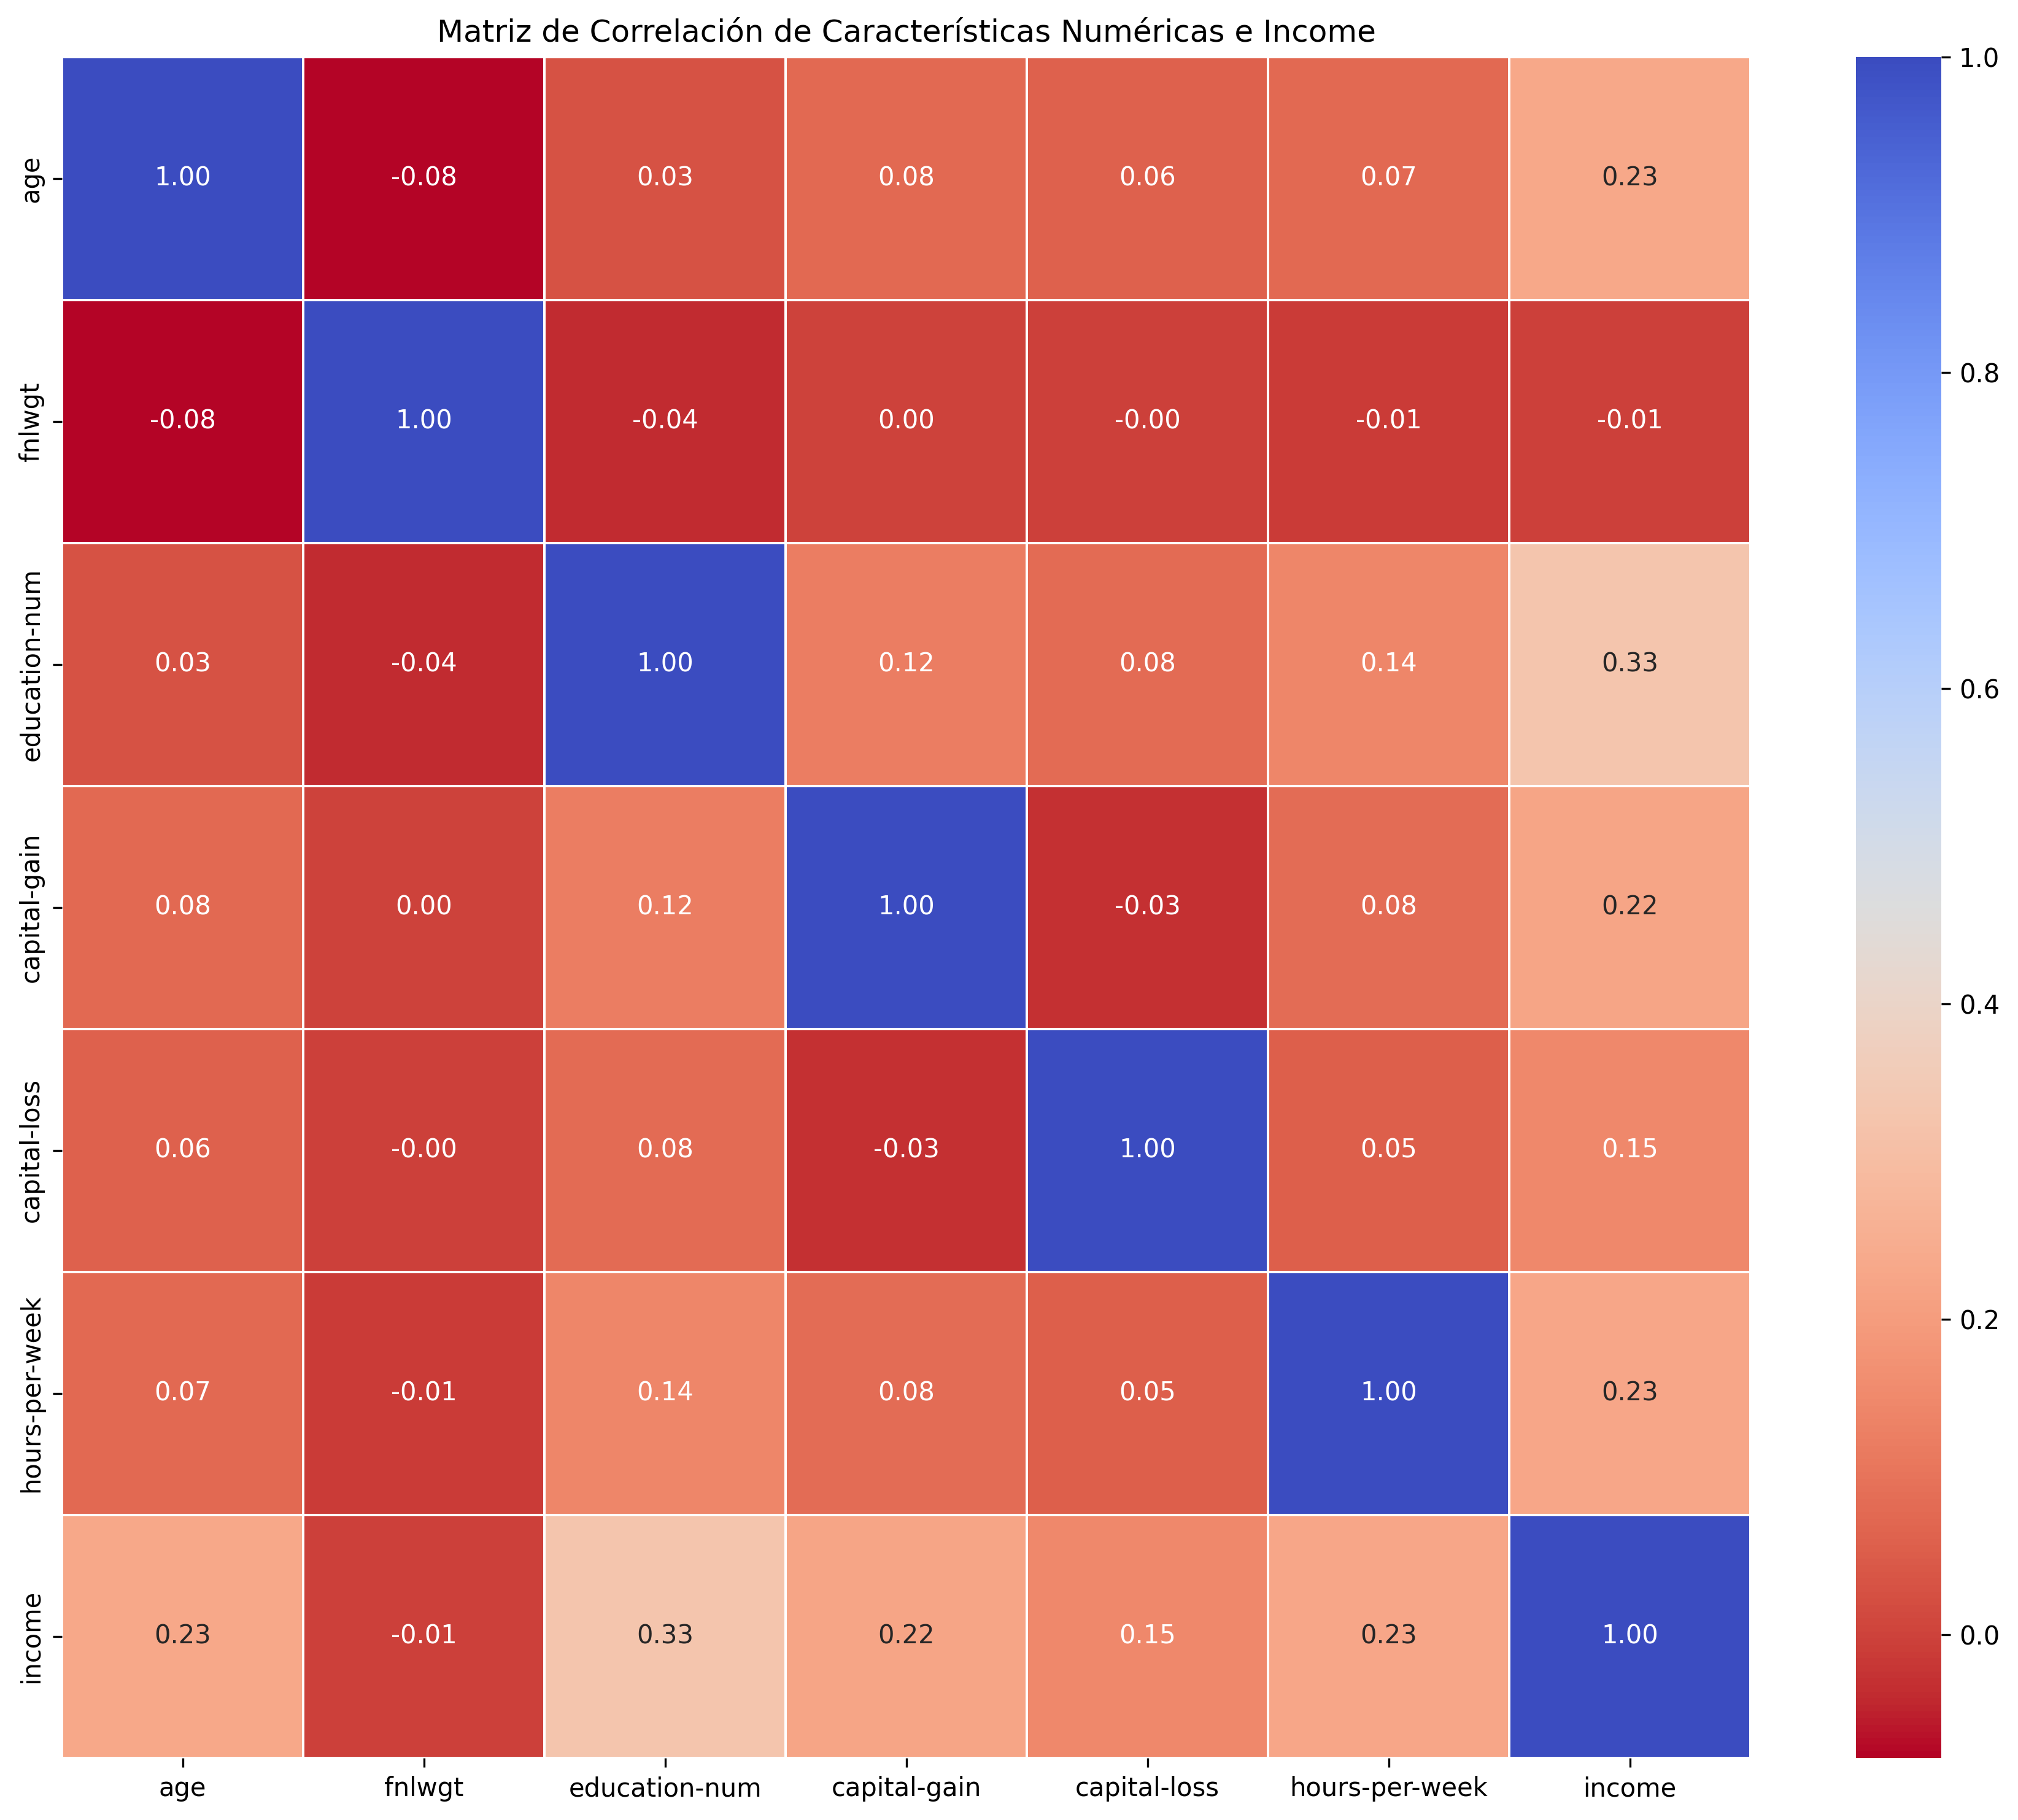
\includegraphics[width=0.8\textwidth]{correlation_matrix_numerical_income.png}
        \caption{Matriz de correlación entre variables numéricas y \texttt{income}.}
        \label{fig:correlation_matrix}
      \end{figure}

      La matriz de correlación entre variables numéricas y \emph{income}, codificada como binaria, muestra asociaciones bajas 
      a moderadas: \emph{education-num}, \emph{hours-per-week} y \emph{age} presentan señales útiles, mientras que \emph{capital-gain} 
      y \emph{capital-loss} aportan información localizada en sus colas. El mapa de calor confirma que no hay colinealidades severas entre 
      predictores numéricos, lo que favorece modelos lineales y árboles sin necesidad de selección por multicolinealidad.
      \vfil

      \item \textbf{Diagramas de dispersión.}
      \begin{figure}[H]
        \centering
        \includegraphics[width=0.95\textwidth]{pairplot_numerical_income.png}
        \caption{Diagramas de dispersión entre variables numéricas y \texttt{income}.}
        \label{fig:scatter_matrix_income}
      \end{figure}

      En los diagramas bivariados se observa un solapamiento importante entre clases para buena parte de las combinaciones, con nubes de 
      puntos densas y sin fronteras lineales claras; sin embargo, emergen patrones útiles: valores positivos de \emph{capital-gain} tienden a 
      asociarse más con \texttt{>50K}, y combinaciones como \emph{education-num}–\emph{hours-per-week} o \emph{age}–\emph{hours-per-week} 
      sugieren gradientes donde mayores niveles educativos o más horas trabajadas elevan la probabilidad de altos ingresos. Estas relaciones 
      recomiendan explorar interacciones y transformaciones no lineales de los datos.

      \item \textbf{Regresión logística como clasificador.}

      Con base en los gráficos y estadísticas, se identificaron cuatro variables con mayor capacidad predictiva para la 
      variable objetivo: \texttt{age}, \texttt{education-num}, \texttt{hours-per-week} y \texttt{capital-gain}. Se utilizó regresión logística 
      para clasificar la variable objetivo, probando distintas combinaciones de pares de estas variables para evaluar el desempeño y rendimiento 
      del modelo. Se obtuvieron los siguientes resultados:

      \begin{table}[H]
        \centering
        \small
        \begin{tabular}{lccccc}
          \toprule
          \textbf{Pareja} & \textbf{Accuracy} & \textbf{Macro P} & \textbf{Macro R} & \textbf{Macro F1} & \textbf{Weighted F1} \\
          \midrule
          (age, education-num)           & 0.7860 & 0.71 & 0.61 & 0.63 & 0.75 \\
          (age, hours-per-week)          & 0.7550 & 0.60 & 0.52 & 0.50 & 0.69 \\
          (age, capital-gain)            & 0.7934 & 0.78 & 0.59 & 0.60 & 0.74 \\
          (education-num, hours-per-week)& 0.7863 & 0.73 & 0.59 & 0.60 & 0.74 \\
          (education-num, capital-gain)  & \textbf{0.8081} & \textbf{0.81} & \textbf{0.62} & \textbf{0.64} & \textbf{0.77} \\
          (hours-per-week, capital-gain) & 0.7952 & 0.78 & 0.60 & 0.61 & 0.75 \\
          \bottomrule
        \end{tabular}
        \caption{Resumen global por pareja}
        \label{tab:resumen_global_parejas}
      \end{table}

      \begin{table}[H]
        \centering
        \small
        \begin{tabular}{lccc}
          \toprule
          \textbf{Pareja} & \textbf{Precision (>50K)} & \textbf{Recall (>50K)} & \textbf{F1 (>50K)} \\
          \midrule
          (age, education-num)            & 0.62 & \textbf{0.27} & 0.38 \\
          (age, hours-per-week)           & 0.44 & 0.08          & 0.14 \\
          (age, capital-gain)             & 0.76 & 0.20          & 0.32 \\
          (education-num, hours-per-week) & 0.66 & 0.22          & 0.33 \\
          (education-num, capital-gain)   & \textbf{0.81} & 0.26 & \textbf{0.39} \\
          (hours-per-week, capital-gain)  & 0.76 & 0.21          & 0.33 \\
          \bottomrule
        \end{tabular}
        \caption{Desempeño en la clase $>50$K}
        \label{tab:minoritaria_parejas}
      \end{table}

      Entre las parejas evaluadas, \texttt{(education-num, capital-gain)} alcanza el mejor desempeño global con una \emph{accuracy} de 0.8081 
      y el mayor \emph{macro F1} (0.64), además del mejor \emph{weighted F1} (0.77). Esto significa que juntar el nivel educativo con las ganancias de capital 
      permite distinguir mejor entre quienes ganan más y menos de 50K. En segundo lugar quedan \texttt{(hours-per-week, capital-gain)} y 
      \texttt{(age, capital-gain)}, ambas alrededor de 0.79–0.80 de \emph{accuracy} y \emph{macro F1} en el rango 0.60–0.61, lo que sugiere que 
      \texttt{capital-gain} aporta gran parte de la separación y que el segundo predictor (edad u horas) añade una ganancia moderada pero real. 
      La pareja \texttt{(age, hours-per-week)} es la menos efectiva, con \emph{accuracy} 0.7550 y un \emph{macro F1} de 0.50, mostrando además el 
      peor recobrado de la clase minoritaria.

      Todas las parejas muestran una clara desigualdad: para \texttt{<=50K} el \emph{recall} ronda 0.97–0.98, mientras que para \texttt{>50K} casi nunca 
      pasa de 0.27. La mejor recuperación de \texttt{>50K} aparece con \texttt{(age, education-num)} (\emph{recall} 0.27), seguida de \texttt{(education-num, capital-gain)} 
      (0.26). Aun así, \texttt{(education-num, capital-gain)} logra a la vez \emph{precision} alta para \texttt{>50K} (0.81) y el mejor equilibrio general; en cambio, 
      \texttt{(age, education-num)} sube el \emph{recall} pero con \emph{precision} menor (0.62) y peor \emph{macro F1}. Esto sugiere que el límite de decisión del modelo 
      favorece a la clase mayoritaria y que la señal de \texttt{capital-gain} es “limpia” (pocos falsos positivos) pero poco común (bajo \emph{recall}). Probar con ajustar 
      ese límite, dar más peso a \texttt{>50K} o crear variables simples (p. ej., un indicador \texttt{capital-gain>0} y una versión logarítmica) podría aumentar el \emph{recall} 
      de \texttt{>50K} sin perder mucha \emph{precision}.

      \texttt{(education-num, capital-gain)} ofrece el mejor equilibrio: mayor \emph{accuracy} (exactitud) y \emph{macro F1}, y detecciones de \texttt{>50K} de 
      “buena calidad” (alta \emph{precision}, 0.81), aunque con \emph{recall} moderado (0.26). \texttt{(hours-per-week, capital-gain)} y \texttt{(age, capital-gain)} 
      confirman que \texttt{capital-gain} es la variable que más separa las clases: mantienen \emph{precision} alta para \texttt{>50K} (0.76 en ambos casos) pero 
      \emph{recall} bajo (0.21–0.20). \texttt{(age, education-num)} logra el mayor \emph{recall} en \texttt{>50K} (0.27), a costa de \emph{precision} más baja (0.62) y 
      menor \emph{macro F1}; sigue siendo útil si la prioridad es “no perder” tantos casos positivos. \texttt{(education-num, hours-per-week)} queda en un punto intermedio y 
      estable, mientras que \texttt{(age, hours-per-week)} se rezaga por su \emph{recall} de 0.08 en \texttt{>50K}.

      Si se busca buen desempeño general y pocas falsas alarmas en \texttt{>50K}, \texttt{(education-num, capital-gain)} es la mejor base.
      Si se quiere aumentar el \emph{recall} de \texttt{>50K}, podría moverse el umbral de decisión y/o da más peso a esa clase, sobre todo en parejas 
      con \texttt{capital-gain}. Por último, añadir una tercera variable (p. ej., \texttt{age} o \texttt{hours-per-week}) probablemente ayudaría a mejorar el 
      \emph{recall} de \texttt{>50K}, siempre que también ajustes el umbral o el peso entre clases.
    \end{itemize}

    \item \textbf{Arbol de decisión como clasificador.}
    
    \begin{table}[H]
      \centering
      \small
        \begin{tabular}{lcccc}
        \toprule
        \textbf{Clase} & \textbf{Precisión} & \textbf{Recall} & \textbf{F1} & \textbf{Soporte} \\
        \midrule
        $\leq$50K & 0.89 & 0.88 & 0.88 & 7422 \\
        $>$50K    & 0.62 & 0.64 & 0.63 & 2336 \\
        \midrule
        \textbf{Accuracy} & \multicolumn{4}{c}{\textbf{0.8216}} \\
        \midrule
        \textbf{Macro promedio}    & 0.75 & 0.76 & 0.76 & 9758 \\
        \textbf{Promedio ponderado} & 0.82 & 0.82 & 0.82 & 9758 \\
        \bottomrule
        \end{tabular}
        \caption{Desempeño del clasificador en el conjunto de prueba}
        \label{tab:clasificador_global}
    \end{table}
    
    El modelo alcanza una precisión general del 82.16\%, lo que indica un buen desempeño global. En la clase menor a 50K, los aciertos 
    son muy altos y constantes (alrededor de 0.88 en todas las métricas), señal de que el modelo identifica bien a quienes ganan hasta 50K. 
    La clase >50K que suele ser la más difícil de predecir muestra un equilibrio sano: cuando el modelo dice que alguien gana más de 50K acierta 62\% 
    de las veces (precisión), y además encuentra 64\% de las personas que realmente están en ese grupo (recuperación). El promedio entre 
    clases (macro) ronda 0.75–0.76, lo que confirma que el rendimiento no depende únicamente de la clase grande; hay un balance razonable 
    entre ambas.

    \begin{itemize}
      \item \textbf{Experimentado con diferentes hiperparámetros.}
      
      \begin{table}[H]
        \centering
        \small
          \begin{tabular}{lcccc}
          \toprule
          \textbf{Clase} & \textbf{Precisión} & \textbf{Recall} & \textbf{F1} & \textbf{Soporte} \\
          \midrule
          $\leq$50K & 0.89 & 0.94 & 0.91 & 7422 \\
          $>$50K    & 0.78 & 0.61 & 0.68 & 2336 \\
          \midrule
          \textbf{Accuracy} & \multicolumn{4}{c}{\textbf{0.8651}} \\
          \midrule
          \textbf{Promedio macro}     & 0.83 & 0.78 & 0.80 & 9758 \\
          \textbf{Promedio ponderado} & 0.86 & 0.87 & 0.86 & 9758 \\
          \bottomrule
          \end{tabular}
        \caption{Desempeño del Árbol de Decisión optimizando hiperparámetros}
        \label{tab:dt_gridsearch_test}
      \end{table}

      El clasificador optimizado alcanzó una precisión global de 86.51\% en el conjunto de prueba, 
      lo que indica un desempeño sólido en términos generales. La clase \(\leq 50\text{K}\) presenta métricas altas (precisión 0.89, recall 0.94 y F1 0.91), 
      evidenciando una identificación consistente de esta categoría. Para la clase \(>50\text{K}\) se observa un equilibrio 
      favorable entre aciertos y cobertura (precisión 0.78 y recall 0.61; F1 0.68), lo que sugiere que el modelo es selectivo al predecir ingresos altos y, 
      al mismo tiempo, recupera una proporción significativa de los casos verdaderamente positivos. Los promedios macro (F1 = 0.80) y ponderado (F1 = 0.86) 
      refuerzan la idea de un rendimiento equilibrado entre ambas clases, sin depender exclusivamente de la mayoritaria. La búsqueda de hiperparámetros exploró 
      combinaciones de \texttt{max\_depth} y \texttt{min\_samples\_split} con validación cruzada, favoreciendo una configuración que controla la complejidad del árbol 
      y mejora la generalización. La mejor configuración de hiperparámetros encontrada fue: \texttt{max\_depth = 10}, \texttt{min\_samples\_split = 20}.

      Se intentó generar el arbol de decisión con todas las reglas evaluadas, sin embargo, es visualmente incomodo, porque unas reglas se solapan con otras 
      difucultando su legibilidad.
    \end{itemize}

    \item \textbf{Clasificador K- Vecinos más cercanos.}
      \begin{table}[H]
        \centering
        \small
          \begin{tabular}{lcccc}
            \toprule
            \textbf{Clase} & \textbf{Precision} & \textbf{Recall} & \textbf{F1-score} & \textbf{Soporte} \\
            \midrule
            <=50K & 0.82 & 0.91 & 0.86 & 7422 \\
            >50K  & 0.56 & 0.34 & 0.43 & 2336 \\
            \midrule
            \textbf{Accuracy}     & \multicolumn{4}{c}{0.78} \\
            \textbf{Macro avg}    & 0.69 & 0.63 & 0.64 & 9758 \\
            \textbf{Weighted avg} & 0.75 & 0.78 & 0.76 & 9758 \\
            \bottomrule
          \end{tabular}
          \caption{Resultados del modelo KNN}
      \end{table}

      El modelo KNN alcanzó una \emph{accuracy} de 0.78, mostrando un buen desempeño para la clase mayoritaria (\texttt{<=50K}, 
      con \emph{recall} 0.91 y \emph{precision} 0.82), pero limitaciones claras en la clase minoritaria (\texttt{>50K}, con \emph{recall} 0.34 y 
      \emph{precision} 0.56). En general, el modelo tiende a favorecer la detección de la clase más común, lo cual se refleja en un \emph{macro F1} 
      relativamente bajo (0.64) frente a un \emph{weighted F1} más alto (0.76). Esto indica que, si bien KNN es confiable para predecir ingresos menores 
      o iguales a 50K, requiere ajustes en hiperparámetros, balanceo de clases o el uso de variables adicionales para mejorar la cobertura en 
      la clase \texttt{>50K}. Para este ejercicio se usó un número de vecinos (k) de 5.

      \begin{itemize}
        \item \textbf{Probando diferentes K.}
        
        % Gráfico desempeño diferentes KNN
        \begin{figure}[H]
          \centering
          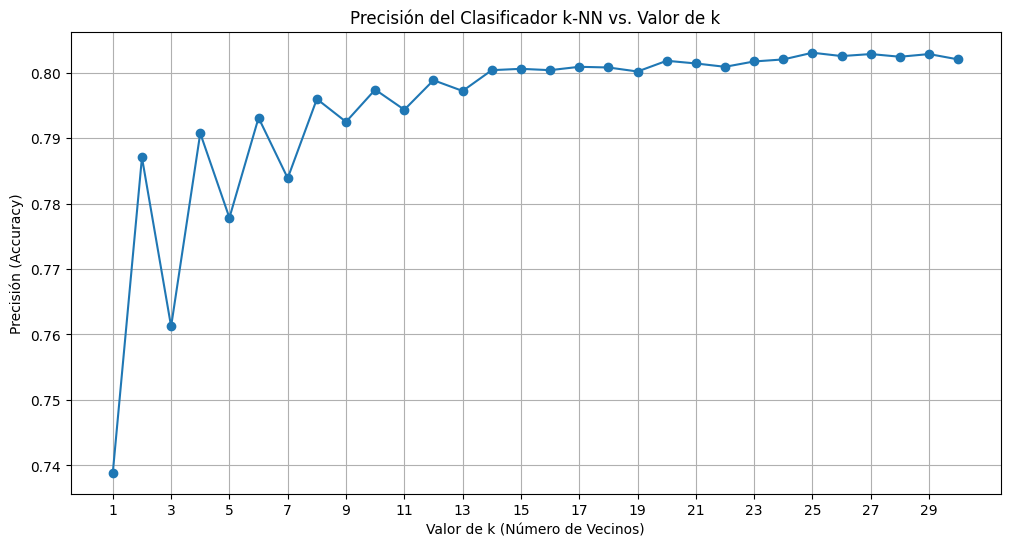
\includegraphics[width=0.6\textwidth]{knn_accuracy_vs_k.png}
          \caption{Desempeño del clasificador con diferentes K}
          \label{fig:knns}
        \end{figure}

        La gráfica evidencia que el clasificador KNN con \(k=1\) presenta la menor \emph{accuracy} (0.74), reflejando tal vez un ajuste excesivo 
        a los datos de entrenamiento. A medida que el número de vecinos aumenta, la precisión mejora de forma rápida y alcanza valores 
        cercanos a 0.79 en torno a \(k=5\)–\(k=7\). A partir de \(k=15\), la \emph{accuracy} se estabiliza alrededor de 0.80–0.81, mostrando 
        un comportamiento más consistente y robusto. En general, los valores intermedios y altos de \(k\) proporcionan el mejor desempeño 
        y un modelo más confiable. El impacto de \(k\) en el clasificador es claro: con valores bajos, el modelo es muy sensible y tiende a sobreajustar; 
        con valores altos, se logra mayor estabilidad pero también se suavizan las fronteras de decisión. Por ello, un rango intermedio 
        (entre 15 y 25 vecinos) resulta el más adecuado, pues equilibra la variabilidad del modelo con su capacidad de generalización.

        Los resultados mostrados en la \Cref{fig:knns} se realizaron sobre el dataset de prueba, previamente habiendo entrenado el modelo con el 
        dataset de entrenamiento.
      \end{itemize}

      \item \textbf{Análisis comparativo.}
      \begin{itemize}
        \item \textbf{Comparación de rendimiento de los modelos.}
        
        En la Tabla~\ref{tab:comparativa_modelos} se presentan los resultados globales de los tres modelos implementados: clasificador 
        basado en reglas, árbol de decisión y KNN. Se reportan las métricas de \textit{accuracy}, F1 macro y F1 ponderado, así como las 
        principales observaciones respecto a la clase minoritaria (>50K).

        \begin{table}[H]
          \centering
          \small
          \resizebox{\textwidth}{!}{%
            \begin{tabular}{lccccl}
              \toprule
              \textbf{Modelo} & \textbf{Accuracy} & \textbf{Macro F1} & \textbf{Weighted F1} & \textbf{Recall (>50K)} & \textbf{Observaciones} \\
              \midrule
              Reglas (education-num, capital-gain) & 0.81 & 0.64 & 0.77 & 0.26 & Alta precisión (0.81) en >50K, bajo recall. \\
              Árbol de decisión (optimizado)       & 0.87 & 0.80 & 0.86 & 0.61 & Mejor balance global, desempeño robusto. \\
              KNN (k=5)                            & 0.78 & 0.64 & 0.76 & 0.34 & Favorece la clase mayoritaria, pobre en >50K. \\
              \bottomrule
            \end{tabular}
          }
          \caption{Comparación del rendimiento de los modelos.}
          \label{tab:comparativa_modelos}
        \end{table}


        En términos generales, el \textbf{árbol de decisión optimizado} es el clasificador con mejor rendimiento y balance entre clases, 
        alcanzando una exactitud de 86.5\% y un F1 macro de 0.80. El \textbf{clasificador basado en reglas} muestra un desempeño aceptable 
        (accuracy de 81\%), pero con bajo recall para la clase minoritaria. Finalmente, el \textbf{KNN} (evaluado en k = 5) alcanza 78\% de exactitud, aunque 
        presenta un sesgo importante hacia la clase mayoritaria.

        \item \textbf{Ventajas y desventajas en el contexto del dataset.}
        \textbf{Clasificador basado en reglas}

        \begin{itemize}
            \item \textbf{Ventajas:} fácil de interpretar; reglas simples con sentido socioeconómico (educación y capital-gain).
            \item \textbf{Desventajas:} baja capacidad para capturar relaciones complejas; muy bajo recall en la clase >50K.
        \end{itemize}

        \textbf{Árbol de decisión}
        \begin{itemize}
            \item \textbf{Ventajas:} mejor balance entre precisión y recall; interpreta relaciones no lineales y variables categóricas sin gran preprocesamiento; relativamente interpretable.
            \item \textbf{Desventajas:} riesgo de sobreajuste si no se regulan los hiperparámetros; árboles grandes son difíciles de interpretar.
        \end{itemize}

        \textbf{KNN}
        \begin{itemize}
            \item \textbf{Ventajas:} implementación simple; no requiere supuestos estadísticos; buen desempeño con valores intermedios de $k$.
            \item \textbf{Desventajas:} sensible a la escala y al desbalance de clases; bajo recall en la clase >50K; elevado costo computacional en predicción.
        \end{itemize}

        En conclusión, para este conjunto de datos el \textbf{árbol de decisión optimizado} resulta la mejor alternativa, ya que logra un 
        desempeño sólido y balanceado entre las dos clases.
      \end{itemize}

\end{enumerate}

\section{Conclusiones}
Se resumen los hallazgos principales, las limitaciones del análisis y posibles mejoras futuras 
(por ejemplo, técnicas de balanceo de clases o selección de características).

\end{document}
